%-*- program: xelatex -*-        
%-*- program: biber -*-`        
%-*- program: xelatex -*-
\documentclass[11pt]{article}
\usepackage[margin=0.75in]{geometry}            % See geometry.pdf to learn the layout options. There are lots.
\geometry{letterpaper}  
\usepackage{amsmath,textcomp,amssymb,geometry,graphicx,enumerate,upquote,color}
\usepackage{hyperref}
\usepackage{breqn}
\usepackage{float}
\usepackage{tikz}
\usepackage{array}
\usepackage{float}
\usepackage{amsfonts}
\def\Session{Fa ll 2015}
\usepackage[english]{babel}
\title{Drawdown Project - Simulation}
\author{Boying Gong, Xinyue Zhou}
\newenvironment{qparts}{\begin{enumerate}[{(}a{)}]}{\end{enumerate}}
\def\endproofmark{$\Box$}
\newenvironment{proof}{\par{\bf Proof}:}{\endproofmark\smallskip}
\begin{document}
\maketitle

\tableofcontents

\clearpage

\section{Noise term with normal distribution}

To better understand the behaviour of conditional expected drawdown (CED) and the maximum drawdown distribution, we use some simple assumptions and parameters in this section as follows:

\begin{enumerate}
\item Noise terms in the time series model follow Normal distribution with standard deviation of 0.01: $\epsilon \sim N(0, 0.0001)$.
\item Risk measures including volatility, VaR, ES and maximum drawdown are calculated based on simulated time series with path length 1000. The calculation of maximum drawdown is replicated 1000 times in order to obtain the maximum drawdown distribution and its tail mean (CED).
\item All time series parameters in this section range from -0.9 to 0.9. For time series with multiple parameters such as AR(2), ARMA(1, 1), the parameters are cartesian product of arithmetic progressions range from -0.9 to 0.9. Note that to take the stationary of AR and ARMA models into consideration (all moving averages are stationary, but the AR and ARMA model have to meet certain criteria to be stationary), not all parameters in the cartesian product are used in the simulation.
\end{enumerate}

%%%%%%%%%%%%
\subsection{AR(1)} %%%%
%%%%%%%%%%%%

We started from the simplest model AR(1):

\begin{equation}
X_t = \kappa_1X_{t-1} + \epsilon_t
\end{equation}

We simulate AR(1) for various values of the autoregressive parameter for $\kappa_1 \in (-1, 1)$ . Figure \ref{fig:AR1_risk_measures} shows the relationship between AR(1) coefficient and risk measures of interest including ES, VaR, volatility and CED. Note that for AR(1) model, the order one serial correlation is the the value of autoregressive parameter.

CED shows a decreasing trend when $\kappa_1\in(-1, -0.75)$ and an increasing trend when $\kappa_1 \in(-0.75, 1)$. As shown in Figure \ref{fig:AR1_risk_measures}, it becomes feasible for us to distinguish negative and positive serial correlation using the CED values. However, the other 3 risk measures are all symmetric about $\kappa_1 = 0$, and they increase as the absolute values of $\kappa_1$ increases.

For VaR, ES and CED, the derivative of risk measure values to $\kappa_1$ approaches to zero as  $\kappa_1$ goes to 0 and increase as $\kappa_1$ increase. This suggests that the value of this three risk measures can hardly reflect the change of serial correlation when the serial correlation is small. And they perform better when the serial correlation increases. The trend of derivatives reverse for CED. While the change of $\kappa_1$ has a comparatively larger influence around 0, the influence becomes weaker as we move to larger  $\kappa_1$ values.

Figure \ref{fig:AR1_maxDrawdown_dist} shows the maximum drawdown distribution for various $\kappa_1$. Same as revealed in Figure \ref{fig:AR1_risk_measures}, the mean and tail mean of maximum drawdown distribution increases as we increase $\kappa_1$ from negative values to positive values.

Table \ref{table: AR1_return} shows the basic summary statistics of the simulated return sequences. The standard deviation increases as we increase the absolute values of the coefficient. The skewness and kurtosis are close to zeros. Kolmogorov-Smirnov Tests indicate that they all follow normal distribution. 

\begin{figure}[H]
\centering
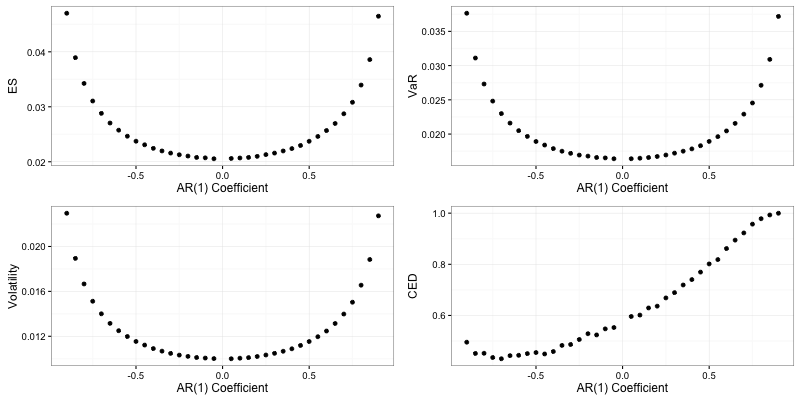
\includegraphics[width = 0.8\textwidth]{../figures/simulation/AR1_risk_measures}
\caption{AR(1): Relationship between auto-correlation coefficients and risk measures}
(Simulation path length: 1000, $\epsilon_t \sim N(0, 0.0001)$)
\label{fig:AR1_risk_measures}
\end{figure}

\begin{figure}[H]
\centering
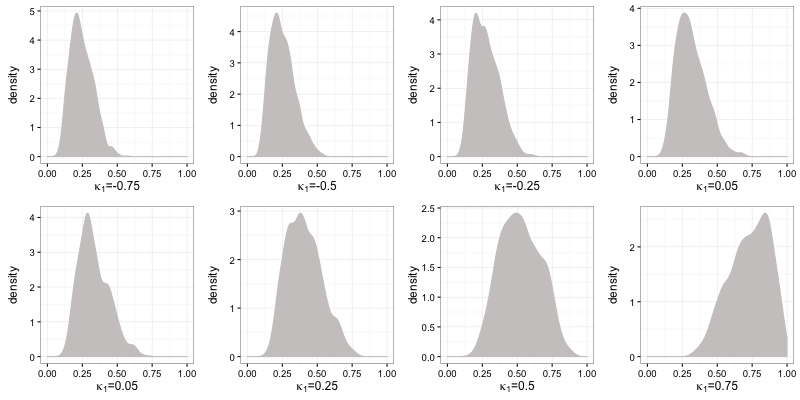
\includegraphics[width = 0.8\textwidth]{../figures/simulation/AR1_maxDrawdown_dist}
\caption{AR(1): Maximum drawdown distribution for various $\kappa_1$ values }
(Empirical distribution, path length = 1000, sample size = 1000, $\epsilon_t \sim N(0, 0.0001)$ )
\label{fig:AR1_maxDrawdown_dist}
\end{figure}

\begin{table}[H]
\centering
\begin{tabular}{|r |r r r r|}
\hline
& Mean & Sd & Skewness & Kurtosis \\
\hline
$\kappa_1 = -0.75$ & 0.0 & 0.015 & 0.009 & 0.032\\
$\kappa_1 = -0.5$ & 0.0 & 0.012 & 0.006 & 0.021\\
$\kappa_1 = -0.25$ & 0.0 & 0.010 & 0.001 & 0.010\\
$\kappa_1 = 0.25$ & 0.0 & 0.010 & -0.009 & 0.004\\
$\kappa_1 = 0.5$ & 0.0 & 0.012 & -0.012 & -0.008\\
$\kappa_1 = 0.75$ & 0.0 & 0.015 & 0.013 & 0.016\\
\hline
\end{tabular}
\caption{Statistics of simulated distribution of AR(1)}
\label{table: AR1_return}
\end{table}

%%%%%%%%%%%%
\subsection{AR(2)} %%%%
%%%%%%%%%%%%

We then move to model AR(2):

\begin{equation}
X_t = \kappa_1X_{t-1} + \kappa_2X_{t-2}  + \epsilon_t
\end{equation}

Figure \ref{fig:AR2_risk_measures_pos} and \ref{fig:AR2_risk_measures_neg} shows the relationship between order one serial correlation $\rho_1$ and various risk measures. With fixed $\kappa_2$, the relationship between serial correlation and various risk measures are close to AR(1) model. The curve shows some discontinuity mainly because the stationary condition for which we have to drop some possible combination of coefficients. Nevertheless, Figure \ref{fig:AR2_risk_measures_pos} and \ref{fig:AR2_risk_measures_neg} shows more complexity in that as we increase the $\kappa_2$ value, the values of all four risk measures increases.

Figure \ref{fig:AR2_maxDrawdown_dist_kappa2_02} and \ref{fig:AR2_maxDrawdown_dist_kappa2_-02} shows the maximum drawdown distribution as we fix $\kappa_2$ to 0.2 and -0.2 respectively and change $\kappa_1$. Again the maximum drawdown distribution shows monotonicity as we increase $\kappa_1$ from negative to positive for both $\kappa_2 = 0.2 $ and $\kappa_2 = -0.2$. It would be the similar if we fix $\kappa_1$ and examine the maximum drawdown distribution for different $\kappa_2$ values.  

Table \ref{table: AR2_return} shows the summary statistics for the simulated return sequences. As indicated above, the standard deviation value increases as we increase the absolute values of the coefficient. The skewness and kurtosis are close to zeros.

\begin{figure}[H]
\centering
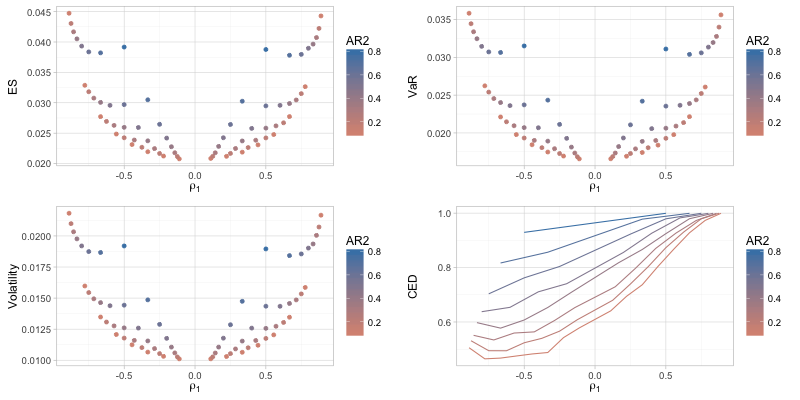
\includegraphics[width = 0.8\textwidth]{../figures/simulation/AR2_risk_measures_pos}
\caption{AR(2): Relationship between serial correlation $\rho_1$ and risk measures ($\kappa_2 > 0$)}
(Simulation path length: 1000, $\epsilon_t \sim N(0, 0.0001)$)
\label{fig:AR2_risk_measures_pos}
\end{figure}

\begin{figure}[H]
\centering
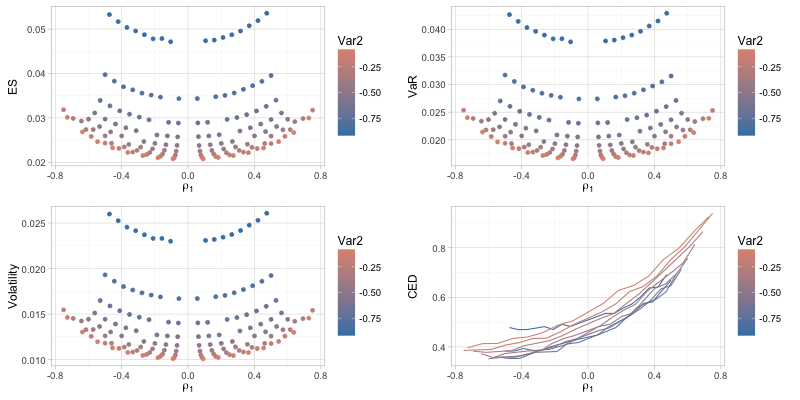
\includegraphics[width = 0.8\textwidth]{../figures/simulation/AR2_risk_measures_neg}
\caption{AR(2): Relationship between serial correlation $\rho_1$ and risk measures ($\kappa_2 < 0$)}
(Simulation path length: 1000, $\epsilon_t \sim N(0, 0.0001)$)
\label{fig:AR2_risk_measures_neg}
\end{figure}

\begin{figure}[H]
\centering
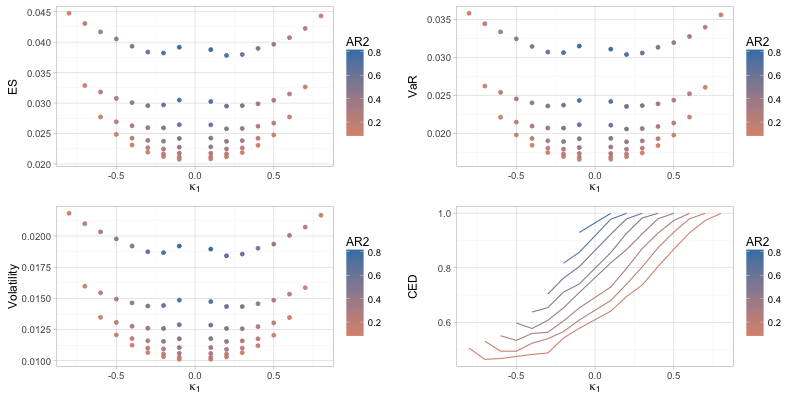
\includegraphics[width = 0.8\textwidth]{../figures/simulation/AR2_risk_measures_pos_coef}
\caption{AR(2): Relationship between model coefficients and risk measures ($\kappa_2 > 0$)}
(Simulation path length: 1000, $\epsilon_t \sim N(0, 0.0001)$)
\label{fig:AR2_risk_measures_pos_coef}
\end{figure}

\begin{figure}[H]
\centering
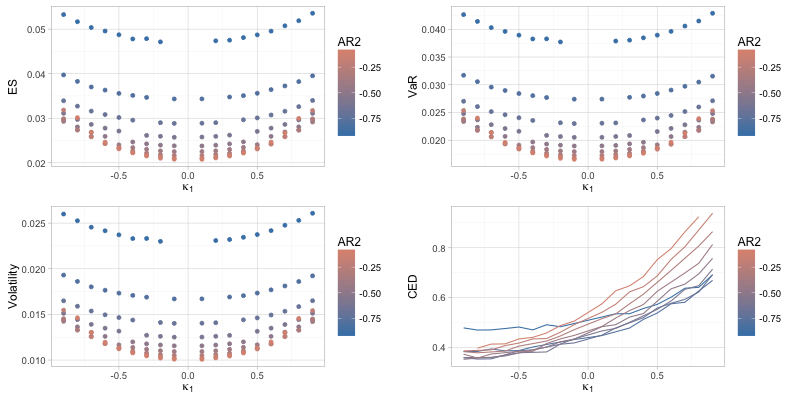
\includegraphics[width = 0.8\textwidth]{../figures/simulation/AR2_risk_measures_neg_coef}
\caption{AR(2): Relationship between model coefficientss and risk measures ($\kappa_2 < 0$)}
(Simulation path length: 1000, $\epsilon_t \sim N(0, 0.0001)$)
\label{fig:AR2_risk_measures_neg_coef}
\end{figure}

\begin{figure}[H]
\centering
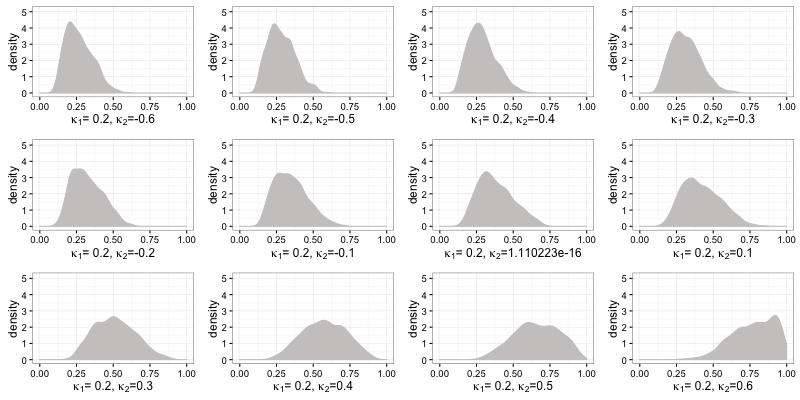
\includegraphics[width = 0.8\textwidth]{../figures/simulation/AR2_maxDrawdown_dist_kappa1_02}
\caption{AR(2): Maximum drawdown distribution for $\kappa_2 = 0.2$}
(Empirical distribution, path length = 1000, sample size = 1000, $\epsilon_t \sim N(0, 0.0001)$ )
\label{fig:AR2_maxDrawdown_dist_kappa2_02}
\end{figure}

\begin{figure}[H]
\centering
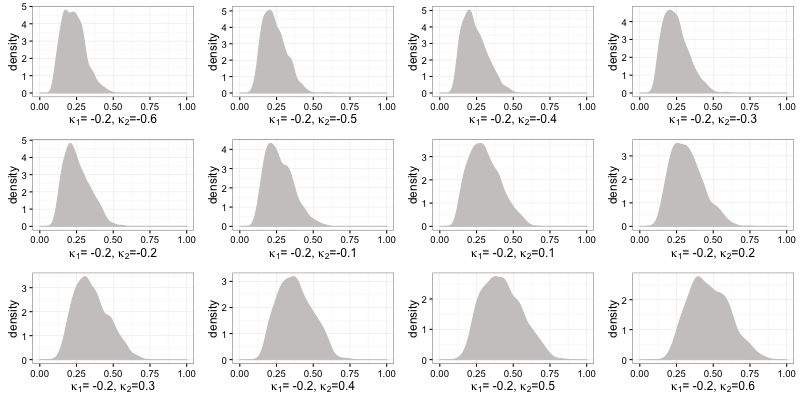
\includegraphics[width = 0.8\textwidth]{../figures/simulation/AR2_maxDrawdown_dist_kappa1_-02}
\caption{AR(2): Maximum drawdown distribution for $\kappa_ = -0.2$}
(Empirical distribution, path length = 1000, sample size = 1000, $\epsilon_t \sim N(0, 0.0001)$ )
\label{fig:AR2_maxDrawdown_dist_kappa2_-02}
\end{figure}

\begin{table}[H]
\centering
\begin{tabular}{|r |r r r r|}
\hline
& Mean & Sd & Skewness & Kurtosis \\
\hline
$\kappa_1 = -0.75, \kappa_2 = 0.2$ & 0.0 & 0.029 & -0.005 & 0.039\\
$\kappa_1 = -0.5, \kappa_2 = 0.2$ & 0.0 & 0.013 & 0.000 & 0.004\\
$\kappa_1 = -0.25, \kappa_2 = 0.2$ & 0.0 & 0.011 & 0.003 & -0.021\\
$\kappa_1 = 0.25, \kappa_2 = 0.2$ & 0.0 &  0.011 & 0.003 & -0.008\\
$\kappa_1 = 0.5, \kappa_2 = 0.2$ & 0.0 & 0.013 & 0.012 & -0.010\\
$\kappa_1 = 0.75, \kappa_2 = 0.2$ & 0.0 &  0.029 & -0.001 & -0.021\\
\hline
\end{tabular}
\caption{Statistics of simulated distribution of AR(2)}
\label{table: AR2_return}
\end{table}

%%%%%%%%%%%%
\subsection{MA(1)} %%%%
%%%%%%%%%%%%

For simplest moving average model MA(1):

\begin{equation}
X_t = \epsilon_t + \theta_1\epsilon_{t-1}
\end{equation}

Figure \ref{fig:MA1_risk_measures_acf1} presents the relationship between four risk measures and serial correlation $\rho_1$. Similar with autoregressive models, CED is a informative risk measures for distinguish positive and negative serial correlations. The curve of $\rho_1$ versus CED is convex for positive serial correlation and concave for negative serial correlation. With means the rate of change of CED to $\rho_1$ is smaller for small serial correlation values and increases for larger serial correlation values. Figure \ref{fig:MA1_risk_measures_coefficient} shows the relationship between risk measures and the moving average coefficient $\theta_1$. Unlike Figure \ref{fig:MA1_risk_measures_acf1}, the MA(1) coefficient shows a relationship close to linear with the change of CED.

Figure \ref{fig:MA1_maxDrawdown_dist} shows the maximum drawdown distribution as we increase $\theta_1$. Same as revealed in the tail mean (CED) of the distribution. The maximum drawdown distribution monotonic increase as $\theta_1$ increases.

\begin{figure}[H]
\centering
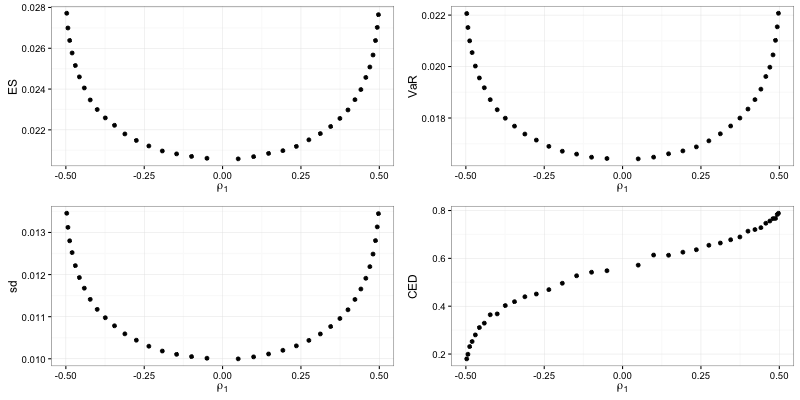
\includegraphics[width = 0.8\textwidth]{../figures/simulation/MA1_risk_measures_acf1}
\caption{MA(1): Relationship between serial correlation $\rho_1$ and risk measures}
(Simulation path length: 1000, $\epsilon_t \sim N(0, 0.0001)$)
\label{fig:MA1_risk_measures_acf1}
\end{figure}

\begin{figure}[H]
\centering
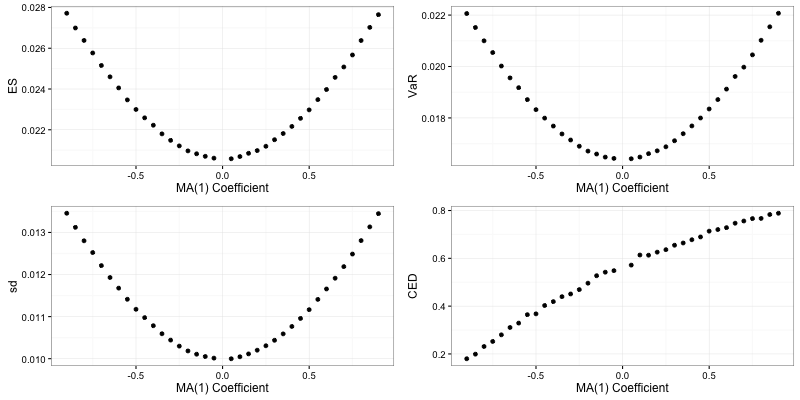
\includegraphics[width = 0.8\textwidth]{../figures/simulation/MA1_risk_measures_coefficient}
\caption{MA(1): Relationship between model coefficient and risk measures}
(Simulation path length: 1000, $\epsilon_t \sim N(0, 0.0001)$)
\label{fig:MA1_risk_measures_coefficient}
\end{figure} 

\begin{figure}[H]
\centering
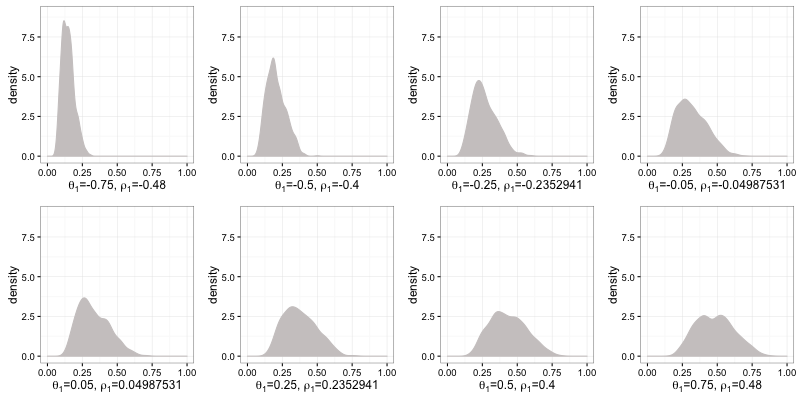
\includegraphics[width = 0.8\textwidth]{../figures/simulation/MA1_maxDrawdown_dist}
\caption{MA(1): Maximum drawdown distribution for various $\theta_1$ values}
(Empirical distribution, path length = 1000, sample size = 1000, $\epsilon_t \sim N(0, 0.0001)$ )
\label{fig:MA1_maxDrawdown_dist}
\end{figure}

\begin{table}[H]
\centering
\begin{tabular}{|r |r r r r|}
\hline
& Mean & Sd & Skewness & Kurtosis \\
\hline
$\theta_1 = -0.75$ & 0.0 & 0.012 & -0.002 & -0.008\\
$\theta_1 = -0.5$ & 0.0 & 0.011 & -0.004 & -0.009\\
$\theta_1 = -0.25$ & 0.0 &  0.010 &  0.001 & -0.020\\
$\theta_1 = 0.25$ & 0.0 &  0.010 & 0.011 & 0.023\\
$\theta_1 = 0.5$ & 0.0 & 0.011 & 0.000 & 0.006\\
$\theta_1 = 0.75$ & 0.0 & 0.013 & -0.003 & 0.012\\
\hline
\end{tabular}
\caption{Statistics of simulated distribution of MA(1)}
\label{table: MA1_return}
\end{table}

%%%%%%%%%%%%%%%%%%%%%%%%
\subsection{MA(2)} %%%%
%%%%%%%%%%%%%%%%%%%%%%%%

The expression of MA(2) model is:

\begin{equation}
X_t = \epsilon_t + \theta_1\epsilon_{t-1} + \theta_2\epsilon_{t-2}
\end{equation}

As shown in Figure \ref{fig:MA2_risk_measures_pos} and Figure \ref{fig:AR2_risk_measures_neg}, when fix $\theta_2$, the relationship between serial correlation $\rho_1$ and risk measures resembles that of the MA(1) model. When we increase the absolute values of $\rho_2$, the value of ES, VaR and volatility increases. However, there are more complicated relationship between serial correlation and CED. For positive $\theta_2$, CED increase as $\theta_2$ increases. The pattern seems less interpretable for negative $\theta_2$ values. 

Figure \ref{fig:MA2_maxDrawdown_dist_theta1_02} shows the change of maximum drawdown distribution when we fix $\theta_1=0.2$, and Figure \ref{fig:MA2_maxDrawdown_dist_theta2_02} shows the maximum drawdown distribution when we fix $\theta_2=0.2$. When fixing one parameter and change the other parameter value from negative to positive, the maximum drawdown distributions are monotonic increasing, which indicates that the tail mean of the distribution (CED) increases.

Same as the AR(1), AR(2), and MA(1) model above, the mean, skewness and kurtosis is small for our simulated return sequences. The standard deviation increase as we increase the absolute value of the coefficient, which can be explained by the theoretical calculation.

\begin{figure}[H]
\centering
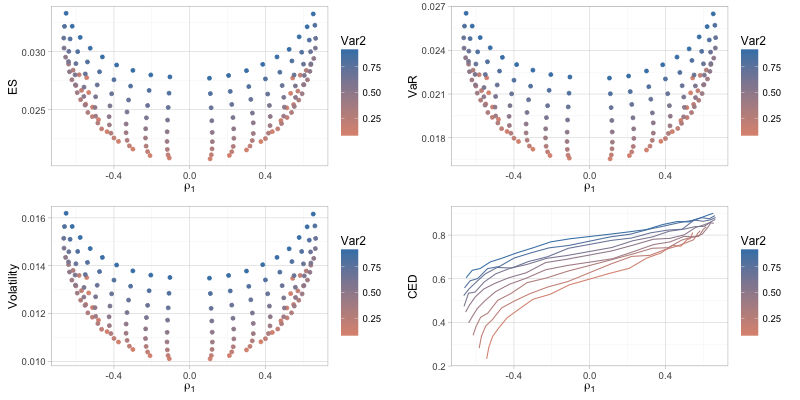
\includegraphics[width = 0.8\textwidth]{../figures/simulation/MA2_risk_measures_pos}
\caption{MA(2): Relationship between serial correlation $\rho_1$ and risk measures ($\theta_2>0$)}
(Simulation path length: 1000, $\epsilon_t \sim N(0, 0.0001)$)
\label{fig:MA2_risk_measures_pos}
\end{figure}

\begin{figure}[H]
\centering
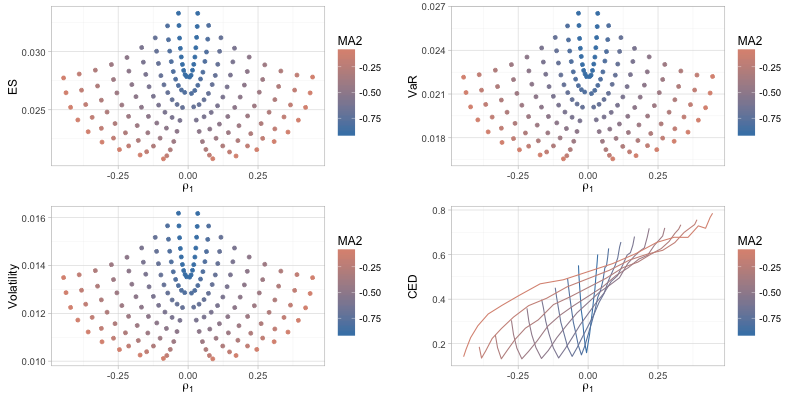
\includegraphics[width = 0.8\textwidth]{../figures/simulation/MA2_risk_measures_neg}
\caption{MA(2): Relationship between serial correlation $\rho_1$ and risk measures ($\theta_2<0$)}
(Simulation path length: 1000, $\epsilon_t \sim N(0, 0.0001)$)
\label{fig:MA2_risk_measures_neg}
\end{figure}

\begin{figure}[H]
\centering
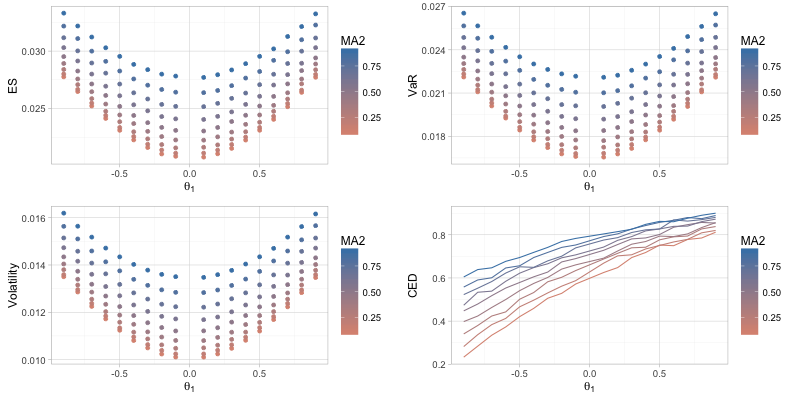
\includegraphics[width = 0.8\textwidth]{../figures/simulation/MA2_risk_measures_pos_coef}
\caption{MA(2): Relationship between model coefficients and risk measures ($\theta_2>0$)}
(Simulation path length: 1000, $\epsilon_t \sim N(0, 0.0001)$)
\label{fig:MA2_risk_measures_pos_coef}
\end{figure}

\begin{figure}[H]
\centering
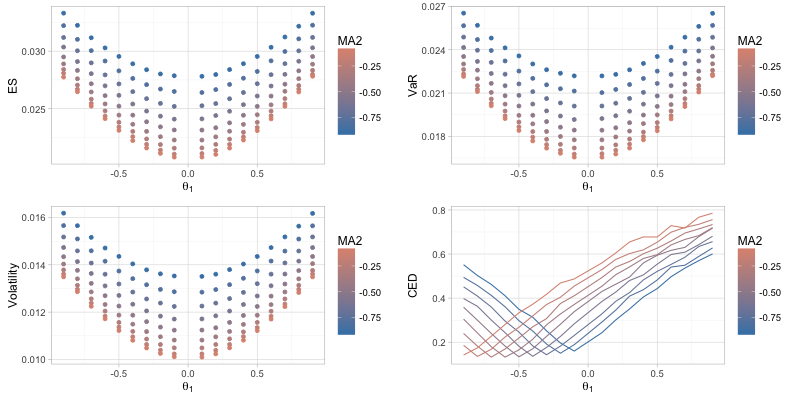
\includegraphics[width = 0.8\textwidth]{../figures/simulation/MA2_risk_measures_neg_coef}
\caption{MA(2): Relationship between model coefficients and risk measures ($\theta_2<0$)}
(Simulation path length: 1000, $\epsilon_t \sim N(0, 0.0001)$)
\label{fig:MA2_risk_measures_neg_coef}
\end{figure}

\begin{figure}[H]
\centering
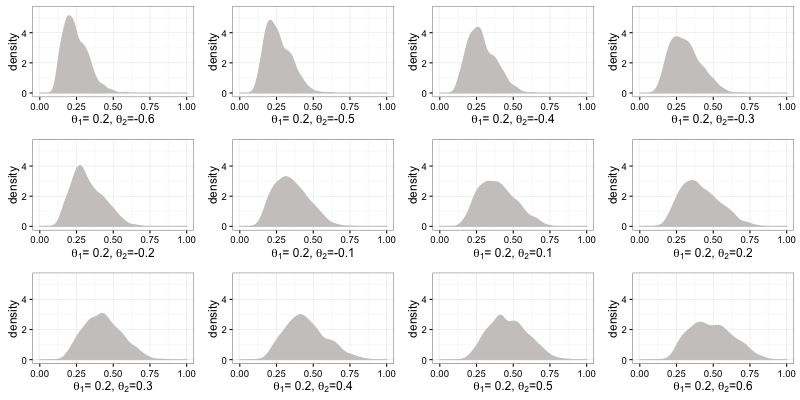
\includegraphics[width = 0.8\textwidth]{../figures/simulation/MA2_maxDrawdown_dist_theta1_02}
\caption{MA(2): Maximum drawdown distribution for $\theta_1 = 0.2$}
(Empirical distribution, path length = 1000, sample size = 1000, $\epsilon_t \sim N(0, 0.0001)$ )
\label{fig:MA2_maxDrawdown_dist_theta1_02}
\end{figure}

\begin{figure}[H]
\centering
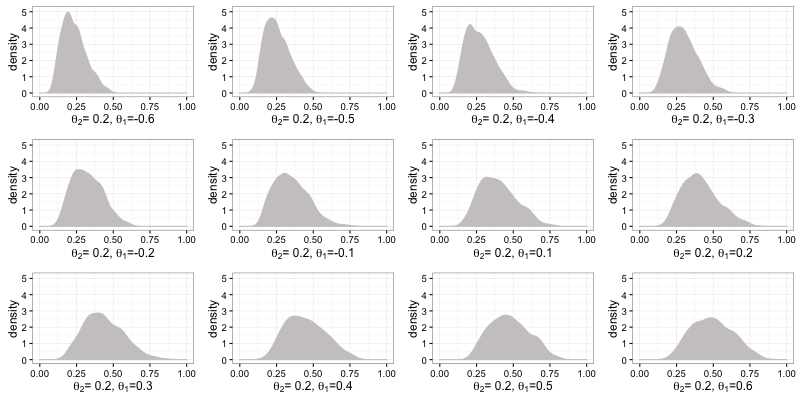
\includegraphics[width = 0.8\textwidth]{../figures/simulation/MA2_maxDrawdown_dist_theta2_02}
\caption{MA(2): Maximum drawdown distribution for $\theta_2 = 0.2$}
(Empirical distribution, path length = 1000, sample size = 1000, $\epsilon_t \sim N(0, 0.0001)$ )
\label{fig:MA2_maxDrawdown_dist_theta2_02}
\end{figure}

\begin{table}[H]
\centering
\begin{tabular}{|r |r r r r|}
\hline
& Mean & Sd & Skewness & Kurtosis \\
\hline
$\theta_1 = -0.75, \theta_2 = 0.2$ & 0.0 & 0.013 & 0.004 & -0.015\\
$\theta_1 = -0.5, \theta_2 = 0.2$ & 0.0 & 0.011 & -0.006 & -0.002\\
$\theta_1 = -0.25, \theta_2 = 0.2$ & 0.0 &  0.011 & -0.004 & -0.012\\
$\theta_1 = 0.25, \theta_2 = 0.2$ & 0.0 &  0.010 & -0.020 & -0.007\\
$\theta_1 = 0.5, \theta_2 = 0.2$ & 0.0 & 0.011 & 0.009 & 0.012\\
$\theta_1 = 0.75, \theta_2 = 0.2$ & 0.0 & 0.013 & -0.015 & 0.025\\
\hline
\end{tabular}
\caption{Statistics of simulated distribution of MA(2)}
\label{table: MA2_return}
\end{table}

%%%%%%%%%%%%%%%%%%%%%%%%%
\subsection{ARMA(1, 1)} %%%%
%%%%%%%%%%%%%%%%%%%%%%%%%

For the most simple ARMA model:

\begin{equation}
X_t = \kappa_1X_{t-1} + \epsilon_t + \theta_1\epsilon_{t-1}
\end{equation}

Figure \ref{fig:AR1MA1_risk_measures_pos} and Figure Figure \ref{fig:AR1MA1_risk_measures_neg} shows the relationship between serial correlation $\rho_1$ and risk measures for positive and negative $\theta_1$ respectively. For positive $\theta_1$, the time series is more likely to be positively correlated while for negative $\theta_1$ it is mode likely to be negative correlated. Interestingly, for positive $\theta_1$ values, the relationship between CED and serial correlation $\rho_1$ is not influenced by the value of $\rho_1$. CED shows an increasing trend as we increase the value of serial correlation. Similar as the above subsections for other time series models, CED is a good tool to distinguish the positive and negative serial correlation.

\begin{figure}[H]
\centering
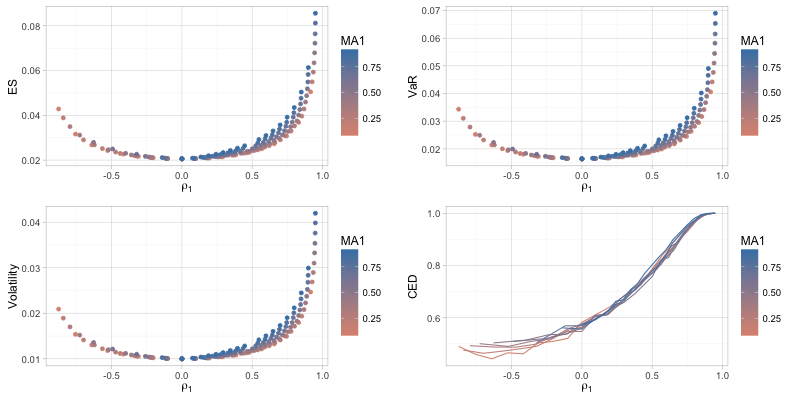
\includegraphics[width = 0.8\textwidth]{../figures/simulation/AR1MA1_risk_measures_pos}
\caption{ARMA(1, 1): Relationship between serial correlation $\rho_1$ and risk measures ($\theta_1>0$)}
(Simulation path length: 1000, $\epsilon_t \sim N(0, 0.0001)$)
\label{fig:AR1MA1_risk_measures_pos}
\end{figure}

\begin{figure}[H]
\centering
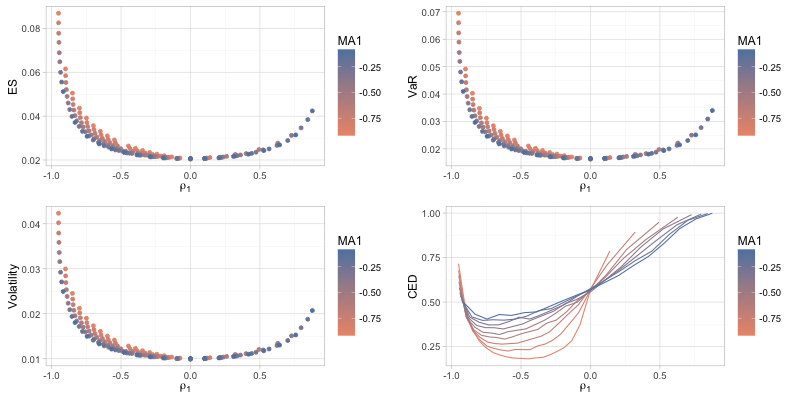
\includegraphics[width = 0.8\textwidth]{../figures/simulation/AR1MA1_risk_measures_neg}
\caption{ARMA(1, 1): Relationship between serial correlation $\rho_1$ and risk measures ($\theta_1>0$)}
(Simulation path length: 1000, $\epsilon_t \sim N(0, 0.0001)$)
\label{fig:AR1MA1_risk_measures_neg}
\end{figure}

\begin{figure}[H]
\centering
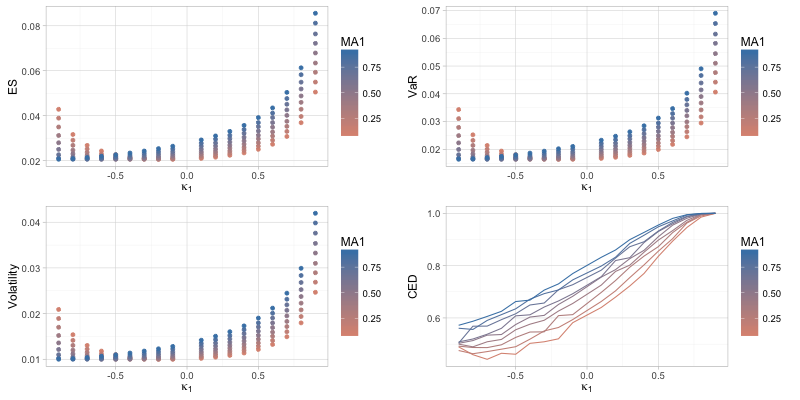
\includegraphics[width = 0.8\textwidth]{../figures/simulation/AR1MA1_risk_measures_pos_coef}
\caption{ARMA(1, 1): Relationship between model coefficient and risk measures ($\theta_1>0$)}
(Simulation path length: 1000, $\epsilon_t \sim N(0, 0.0001)$)
\label{fig:AR1MA1_risk_measures_pos_coef}
\end{figure}

\begin{figure}[H]
\centering
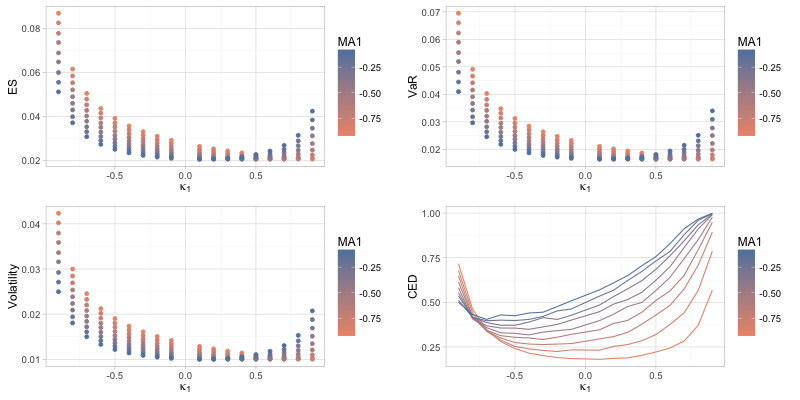
\includegraphics[width = 0.8\textwidth]{../figures/simulation/AR1MA1_risk_measures_neg_coef}
\caption{ARMA(1, 1): Relationship between model coefficient and risk measures ($\theta_1>0$)}
(Simulation path length: 1000, $\epsilon_t \sim N(0, 0.0001)$)
\label{fig:AR1MA1_risk_measures_neg_coef}
\end{figure}



%%%%%%%%%%%%%%%%%%%%%%%%%%%%%%%%%%%%%%%%%%%%%%%%%%
%%%%%%%%%%%%%%%%%%%%%%%%%%%%%%%%%%%%%%%%%%%%%%%%%%
\section{Noise term with student t distribution}
%%%%%%%%%%%%%%%%%%%%%%%%%%%%%%%%%%%%%%%%%%%%%%%%%%

In this section, parameters used are close to what we've encountered in the empirical studies. 
\begin{enumerate}
\item White noise terms are simulated using t-distribution (degree of freedom = 4). Financial return usually have fat-tail distributions.
\item Set path length to 63, which is the number of trading days in three month.
\item Time series parameters all range from -0.3 to 0.3, which is similar to the financial time series data in the real world. Usually financial data does not show strong serial correlation. If we could narrow down our scope to smaller serial correlations we may found that the serial correlation is more closely related with various risk measures.
\end{enumerate}

The relationship between serial correlation and risk measures revealed in this section resembles that of the last section where noise terms follow normal distribution. There are some differences due to the heavy-tail distribution. We illustrate more in the specific model part.

\subsection{AR(1)}

Models using time series with t-distribution white noise show more randomness as shown in Figure \ref{table: T_dist_AR1_return}. The relationship between AR(1) coefficients (which is the serial correlation $\rho_1$) and risk measures is similar to the model with normal distribution. However, the points are not lies perfectly in a curve probably because the heavy tail introduce more randomness of the quantile and tail mean values. 

Table \ref{table: T_dist_AR1_return} shows the summary statistics of the simulated return distribution. Their mean and skewness are close to zero. And they have high kurtosis which implies the fat tail.

\begin{figure}[H]
\centering
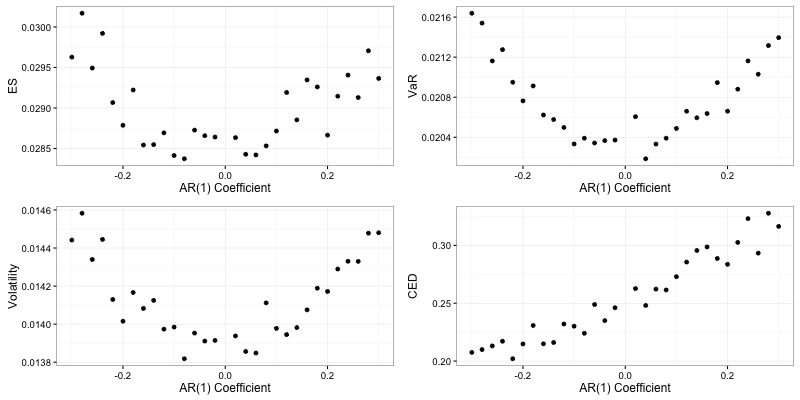
\includegraphics[width = 0.8\textwidth]{../figures/simulation/T_dist_AR1_risk_measures}
\caption{AR(1): Relationship between auto-correlation coefficients and risk measures}
(Simulation path length: 63, $\epsilon_t \sim 0.01T(df = 4)$)
\label{fig:T_dist_AR1_risk_measures}
\end{figure}



\begin{figure}[H]
\centering
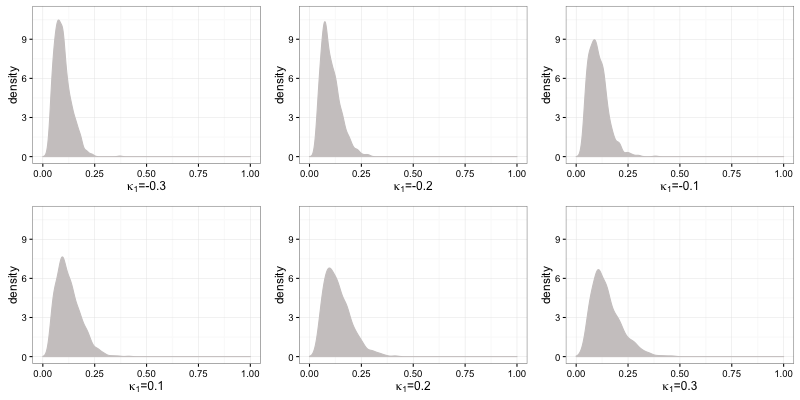
\includegraphics[width = 0.8\textwidth]{../figures/simulation/T_dist_AR1_maxDrawdown_dist}
\caption{AR(1): Maximum drawdown distribution for various $\kappa_1$ values }
(Empirical distribution, path length = 63, sample size = 1000, $\epsilon_t \sim 0.01T(df = 4)$)
\label{fig:T_dist_AR1_maxDrawdown_dist}
\end{figure}


\begin{table}[H]
\centering
\begin{tabular}{|r |r r r r|}
\hline
& Mean & Sd & Skewness & Kurtosis \\
\hline
$\kappa_1 = -0.3$ & 0.0 & 0.015 & -0.53 & 18.8\\
$\kappa_1 = -0.2$ & 0.0 & 0.014 & -0.13 & 6.4\\
$\kappa_1 = -0.1$ & 0.0 & 0.014 & -0.05 & 6.3\\
$\kappa_1 = 0.1$ & 0.0 & 0.014 & -0.30 & 15.8\\
$\kappa_1 = 0.2$ & 0.0 & 0.014 & 0.13 & 7.0\\
$\kappa_1 = 0.3$ & 0.0 & 0.015 & -0.06 & 7.4\\
\hline
\end{tabular}
\caption{Statistics of simulated distribution of AR(1)}
\label{table: T_dist_AR1_return}
\end{table}

\subsection{AR(2)}

Same as presented in the last section, ES, VaR and volatility increases as we increase the absolute values of $\kappa_2$. And CED increases as we change $\kappa_2$ from negative to positive. This shows that CED values are inherently not symmetric not only for the serial correlation but for the coefficients. The summary statistics in Table \ref{table: T_dist_AR2_return} also indicate the fat tail distribution.

\begin{figure}[H]
\centering
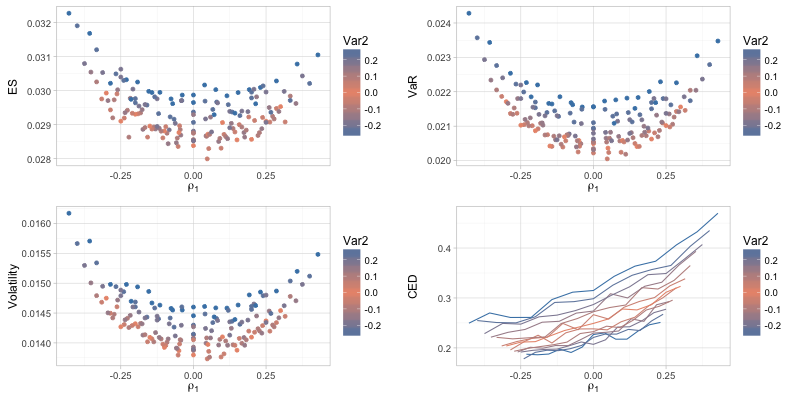
\includegraphics[width = 0.8\textwidth]{../figures/simulation/T_dist_AR2_risk_measures}
\caption{AR(2): Relationship between auto-correlation coefficients and risk measures}
(Simulation path length: 63, $\epsilon_t \sim 0.01T(df = 4)$)
\label{fig:T_dist_AR2_risk_measures}
\end{figure}

\begin{figure}[H]
\centering
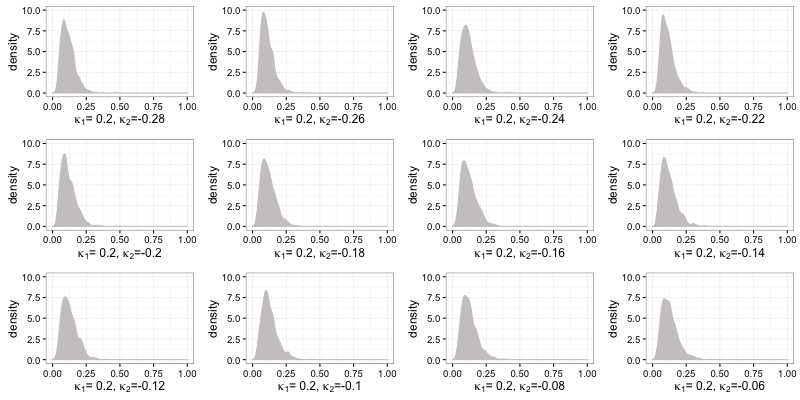
\includegraphics[width = 0.8\textwidth]{../figures/simulation/T_dist_AR2_maxDrawdown_dist_kappa1_02}
\caption{AR(2): Maximum drawdown distribution for various $\kappa_2$ values }
(Empirical distribution, path length = 63, sample size = 1000, $\epsilon_t \sim 0.01T(df = 4)$)
\label{fig:T_dist_AR2_maxDrawdown_dist_kappa1_02}
\end{figure}

\begin{table}[H]
\centering
\begin{tabular}{|r |r r r r|}
\hline
& Mean & Sd & Skewness & Kurtosis \\
\hline
$\kappa_1 = 0.1, \kappa_2 = -0.3$ & 0.0 & 0.015 & -0.024 & 16.7\\
$\kappa_1 = 0.1, \kappa_2 = -0.2$ & 0.0 & 0.014 & -0.030 & 8.0\\
$\kappa_1 = 0.1, \kappa_2 = -0.1$ & 0.0 & 0.014 & -0.261 & 16.7\\
$\kappa_1 = 0.1, \kappa_2 = 0.1$ & 0.0 & 0.014 & -0.461 & 18.2\\
$\kappa_1 = 0.1, \kappa_2 = 0.2$ & 0.0 & 0.014 & 0.028 & 6.0\\
$\kappa_1 = 0.1, \kappa_2 = 0.3$ & 0.0 & 0.015 & -0.009 & 5.8\\
\hline
\end{tabular}
\caption{Statistics of simulated distribution of AR(2)}
\label{table: T_dist_AR2_return}
\end{table}

\subsection{MA(1)}

Again the relationship between serial correlation and risk measures for MA(1) model greatly resembles the relationship in last section for the normal distributed noise term. The difference lies in the large randomness caused by the fat tail. 

\begin{figure}[H]
\centering
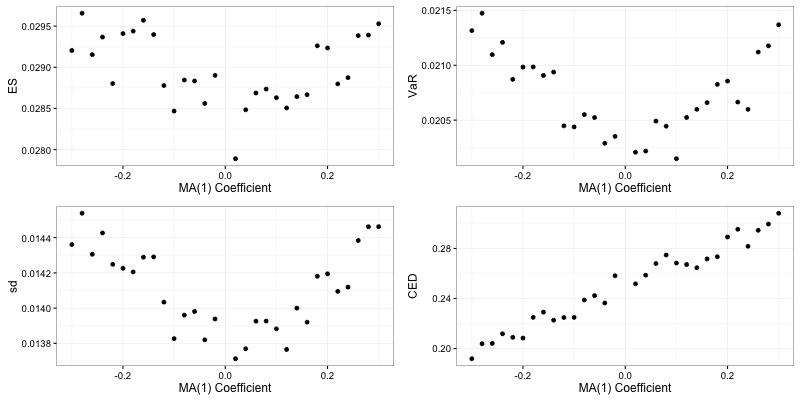
\includegraphics[width = 0.8\textwidth]{../figures/simulation/T_dist_MA1_risk_measures_coefficient.png}
\caption{MA(1): Relationship between serial correlation $\rho_1$ and risk measures}
(Simulation path length: 63, $\epsilon_t \sim 0.01T(df = 4)$)
\label{fig:T_dist_MA1_risk_measures_coefficient}
\end{figure}

\begin{figure}[H]
\centering
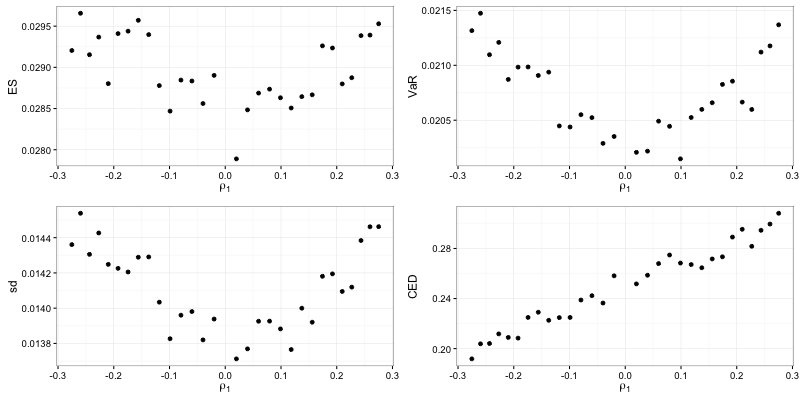
\includegraphics[width = 0.8\textwidth]{../figures/simulation/T_dist_MA1_risk_measures_acf1.png}
\caption{MA(1): Relationship between model coefficient and risk measures}
(Simulation path length: 63, $\epsilon_t \sim 0.01T(df = 4)$)
\label{fig:T_dist_MA1_risk_measures_acf1}
\end{figure} 

\begin{figure}[H]
\centering
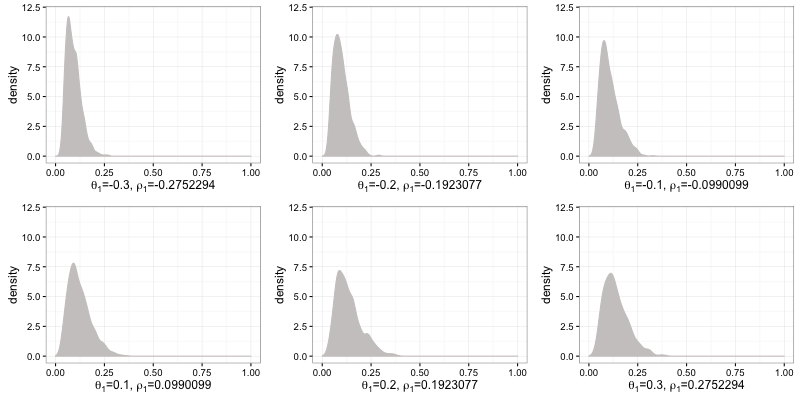
\includegraphics[width = 0.8\textwidth]{../figures/simulation/T_dist_MA1_maxDrawdown_dist}
\caption{MA(1): Maximum drawdown distribution for various $\kappa_1$ values }
(Empirical distribution, path length = 63, sample size = 1000, $\epsilon_t \sim 0.01T(df = 4)$)
\label{fig:T_dist_MA1_maxDrawdown_dist}
\end{figure}

\begin{table}[H]
\centering
\begin{tabular}{|r |r r r r|}
\hline
& Mean & Sd & Skewness & Kurtosis \\
\hline
$\kappa_1 = 0.1, \kappa_2 = -0.3$ & 0.0 & 0.015 & -0.401 & 22.9\\
$\kappa_1 = 0.1, \kappa_2 = -0.2$ & 0.0 & 0.014 & -0.312 & 12.3\\
$\kappa_1 = 0.1, \kappa_2 = -0.1$ & 0.0 & 0.014 & -0.204 & 8.5\\
$\kappa_1 = 0.1, \kappa_2 = 0.1$ & 0.0 & 0.014 & -0.009 & 9.7\\
$\kappa_1 = 0.1, \kappa_2 = 0.2$ & 0.0 & 0.014 & -0.080 & 7.2\\
$\kappa_1 = 0.1, \kappa_2 = 0.3$ & 0.0 & 0.015 & -0.136 & 12.5\\
\hline
\end{tabular}
\caption{Statistics of simulated distribution of MA(1)}
\label{table: T_dist_MA1_return}
\end{table}

\subsection{MA(2)}

Since we have narrowed down our scope to time series coefficients which range between -0.3 and 0.3. Here we can see that for fixed value of $\theta_2$, the relationship between serial correlation and CED is approximately a line. And for the other three risk measures, the relationship seems to have more randomness than using normal distribution. 

\begin{figure}[H]
\centering
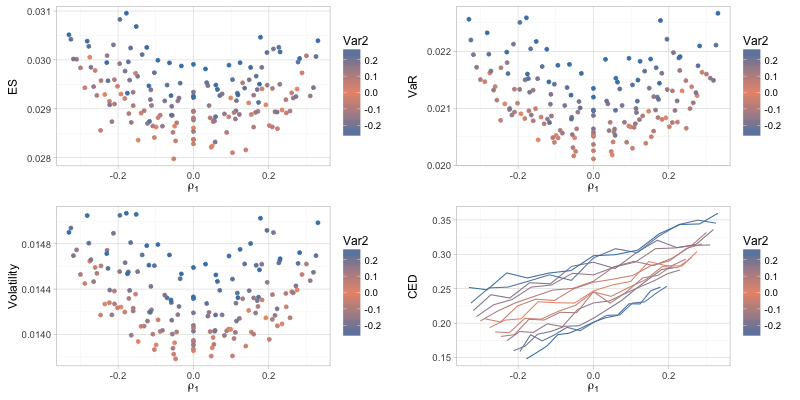
\includegraphics[width = 0.8\textwidth]{../figures/simulation/T_dist_MA2_risk_measures}
\caption{MA(1): Relationship between serial correlation $\rho_1$ and risk measures}
(Simulation path length: 63, $\epsilon_t \sim 0.01T(df = 4)$)
\label{fig:T_dist_MA2_risk_measures}
\end{figure}

\begin{figure}[H]
\centering
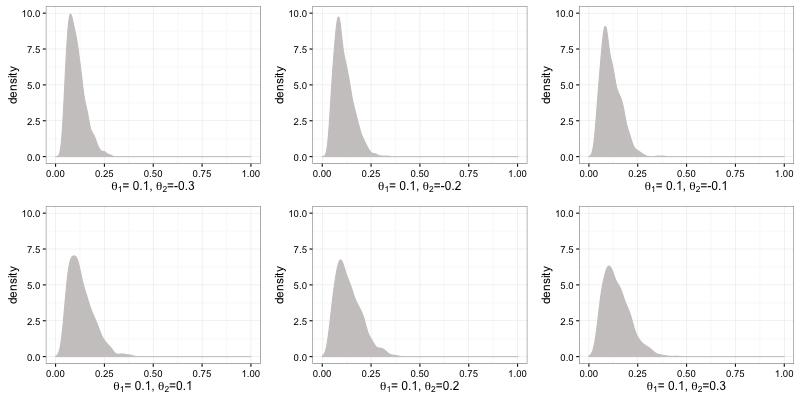
\includegraphics[width = 0.8\textwidth]{../figures/simulation/T_dist_MA2_maxDrawdown_dist_theta1_01}
\caption{MA(1): Maximum drawdown distribution for various $\kappa_1$ values }
(Empirical distribution, path length = 63, sample size = 1000, $\epsilon_t \sim 0.01T(df = 4)$)
\label{fig:T_dist_MA2_maxDrawdown_dist_theta1_01.png}
\end{figure}

\begin{table}[H]
\centering
\begin{tabular}{|r |r r r r|}
\hline
& Mean & Sd & Skewness & Kurtosis \\
\hline
$\kappa_1 = 0.1, \kappa_2 = -0.3$ & 0.0 & 0.015 & -0.204 & 10.7\\
$\kappa_1 = 0.1, \kappa_2 = -0.2$ & 0.0 & 0.015 & 0.162 & 8.9\\
$\kappa_1 = 0.1, \kappa_2 = -0.1$ & 0.0 & 0.014 & -0.229 & 6.2\\
$\kappa_1 = 0.1, \kappa_2 = 0.1$ & 0.0 & 0.014 & -0.220 & 13.3\\
$\kappa_1 = 0.1, \kappa_2 = 0.2$ & 0.0 & 0.015 & 0.117 & 9.7\\
$\kappa_1 = 0.1, \kappa_2 = 0.3$ & 0.0 & 0.015 & -0.097 & 9.9\\
\hline
\end{tabular}
\caption{Statistics of simulated distribution of MA(2)}
\label{table: T_dist_MA2_return}
\end{table}

\subsection{ARMA(1, 1)}

\begin{figure}[H]
\centering
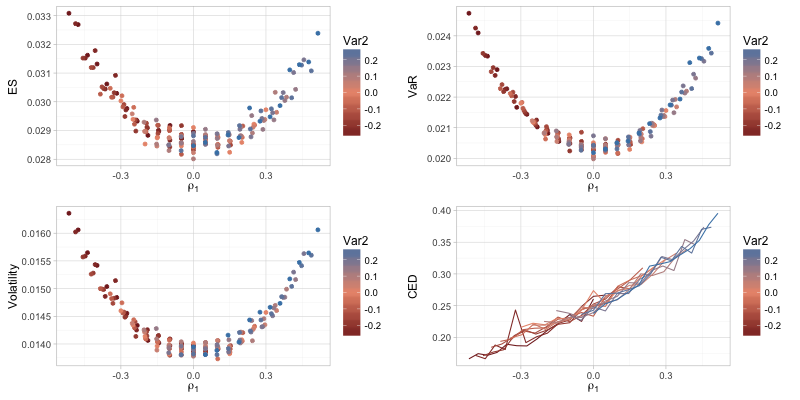
\includegraphics[width = 0.8\textwidth]{../figures/simulation/T_dist_AR1MA1_risk_measures}
\caption{ARMA(1, 1): Relationship between serial correlation $\rho_1$ and risk measures}
(Simulation path length: 63, $\epsilon_t \sim 0.01T(df = 4)$)
\label{fig:T_dist_AR1MA1_risk_measures}
\end{figure}

%%%%%%%%%%%%%%%%%%%%%%%%%%%%%%%%%%%%%%%%%%%%%%%%%%
%%%%%%%%%%%%%%%%%%%%%%%%%%%%%%%%%%%%%%%%%%%%%%%%%%
\section{Simulation with standard error adjusted} %%%%%%
%%%%%%%%%%%%%%%%%%%%%%%%%%%%%%%%%%%%%%%%%%%%%%%%%%

So far our simulation studies are based on fixed distribution of the noise term. For example, for normal distribution noise we use $\epsilon \sim N(0, 0.0001)$ and for t-distribution we use $\epsilon \sim 0.01T(df =4)$. In this section, we standardize the simulated time series by dividing certain factors such that the time series have same standard deviation. 

In our simulation, the standard deviation for each our simulated time series is different. Say for AR(1), the standard deviation of time series $X_t = 0.5  X_{t-1} + \epsilon_t$ and $X_t = 0.1  X_{t-1} + \epsilon_t$ is different since we use the same distribution for $\epsilon_t$. The standard deviation for AR(1) model is :

\begin{equation}
SD(X_t) = \Big(\frac{Var(\epsilon_t)}{1-\kappa_1^2}\Big)^{1/2}
\end{equation}

 Then what if we compare two time series with different distribution of $\epsilon_t$ but the same standard deviation? Since standard deviation is one risk measures (volatility), this equals to fixing other risk measures to one level, say volatility = 1.2\%, and to see how CED changes with the serial correlation. 

 Since our simulation is based on normal distribution of the noise term, volatility would be proportional to ES and VaR, which means fixed volatility also means fixed volatility. 

 Figure \ref{fig:AR1_adjsd} and \ref{fig:MA1_adjsd} shows the result for AR(1) and MA(1) separately. and Figure \ref{fig:aggregated_adjsd} shows the results for AR(2), MA(2) and ARMA(1, 1). There is clearer upward trends than the last two sections. These figures suggests that CED is a better metric in describing the returns with serial correlation. For the same volatility level, CED increases as the serial correlation increases, which means CED captures the changes in serial correlation while volatility, VaR and ES do not. 

\begin{figure}[H]
\centering
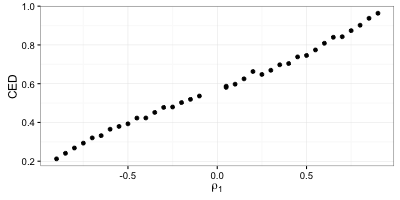
\includegraphics[width = 0.5\textwidth]{../figures/simulation/AR1_adjsd}
\caption{AR(1): Relationship between serial correlation $\rho_1$ and CED with adjusted standard error}
(Simulation path length: 1000)
\label{fig:AR1_adjsd}
\end{figure}

\begin{figure}[H]
\centering
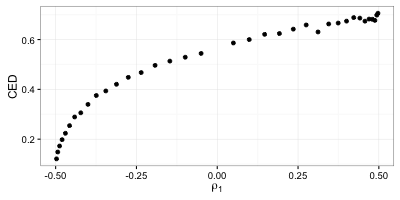
\includegraphics[width = 0.5\textwidth]{../figures/simulation/MA1_adjsd}
\caption{MA(1): Relationship between serial correlation $\rho_1$ and CED with adjusted standard error}
(Simulation path length: 1000)
\label{fig:MA1_adjsd}
\end{figure}

\begin{figure}[H]
\centering
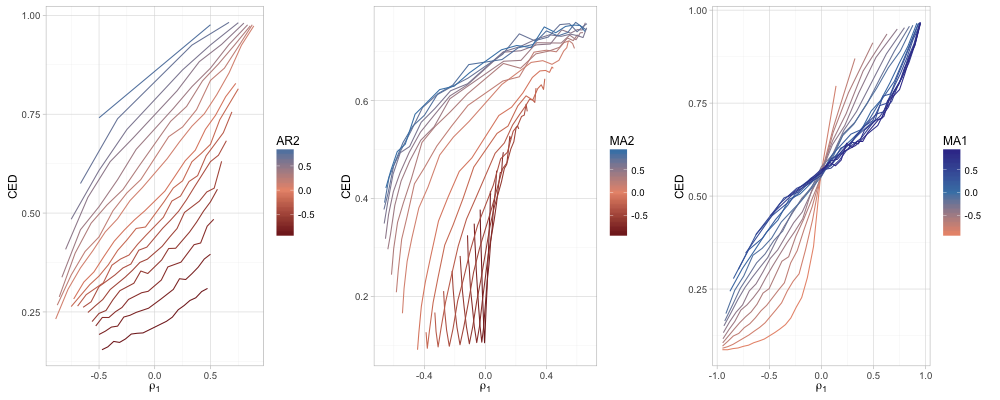
\includegraphics[width = 1\textwidth]{../figures/simulation/aggregated_adjsd}
\caption{Relationship between serial correlation $\rho_1$ and CED with adjusted standard error}
(Simulation path length: 1000, from left to right: AR(2), MA(2), ARMA(1, 1))
\label{fig:aggregated_adjsd}
\end{figure}

\begin{figure}[H]
\centering
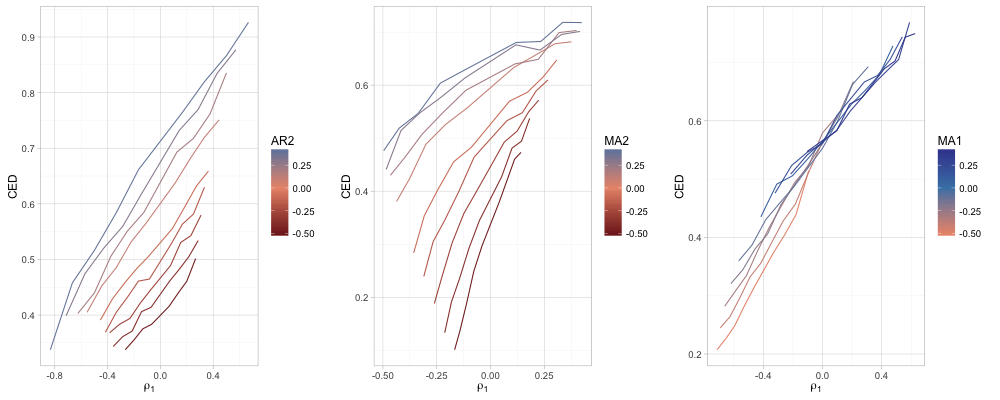
\includegraphics[width = 1\textwidth]{../figures/simulation/aggregated_adjsd_subset}
\caption{Relationship between serial correlation $\rho_1$ and CED with adjusted standard error}
(Simulation path length: 1000, from left to right: AR(2), MA(2), ARMA(1, 1), model coefficient $\in(-0.5, 0.5)$)
\label{fig:aggregated_adjsd_subset}
\end{figure}


%%%%%%%%%%%%%%%%%%%%%%%%%
\section{More Complex noise Term}  %%%%%
%%%%%%%%%%%%%%%%%%%%%%%%%
The previous several sections have already stated general ideas that how magnitude of risk measurements correlated with serial correlation and ARMA coefficients. However, the inspiring results should not encourage us ignore the complexity of the market: it always does not produce such regular time series. The occasional events shock the market and the returns always shows clustered variance. As has been analyzed in the previous reports, a normal way to handle the complex variance in the return is using generalized autoregressive conditional heteroskedasticity (GARCH) model. In this section, common ARMA time series are simulated with GARCH noise term, to which we expect analysis the extent of effect that complex noise term having on the relationship between serial correlation and risk measurements.

\begin{enumerate}
\item At this level, we limit our analysis on GARCH(1,1), for the reason that in the empirical study on thirteen American indices, GARCH(1,1) is good enough catch the variance anomaly in the return.
\item The GARCH model is based on the Gaussian conditional distribution. Although in the empirical study on thirteen American indices, we showed that a student t conditional distribution seems to be more able to approximate the true market, Gaussian enable us to analyze more properties in the return without losing the generality
\item For GARCH(1,1), recall  that:
\[
\sigma^2_t = \omega + \alpha y_{t-1}^2 + \beta \sigma^2_{t-1}
\]
 We choose the potential parameters on the basis of  the study of the American financial indices. In summary, we choose $\omega \in \{10^{-7}, 10^{-8}\}$, $\alpha \in \{0.05, 0.08, 0.11, 0.14, 0.17, 0.20\}$, $\beta  \in \{0.1,0.2,\dots, 0.7\}$.
\end{enumerate}

\subsection{AR(1) + GARCH(1,1)}
How $\omega$, $\alpha$ and $\beta$ affect the magnitude of risk measurement is kind of inconspicuous. As $y_{t-1}^2$, $\sigma_{t-1}^2$ and $\beta$ are positive number, the only thing we can ensure is that all the GARCH parameters are positively correlated with variance, thus the `` risk'' in some sense. However, there are more questions in need of taking care: 1) which parameter within $\omega$, $\alpha$ and $\beta$ are more responsible for the change in risk measurements? 2) Comparing the extent that the risk measurements changing with serial correlation or coefficients, does $\alpha$ and $\beta$ counts a lots?

The Figure \ref{fig:garch_rm_alpha1} verifies our guess. The higher $\omega$, $\alpha$ or $\beta$ are all partial responsible for a highly risk measurements, in general. The eight lines with in the plots are clearly separate into two groups, upper and lower. The higher four curves have a higher $\omega$, which indicates a general magnitude of variance. Therefore, $\omega$ is dominant with in parameters.

ES, VaR and Volatility are monotonically increasing with $alpha$. When the $\beta$ is relatively small, this relationship is almost linear, while when the $\beta$ is large, the relationship is more likely to be a higher order polynomial shape.

In general, the CED has a similar trend with other risk measurements, while it less smoother. Especially, when the $\beta$ is low, $\alpha's$ effect is even more unclear. Showing in the plot is the lowest three lines are twisting together. 
\begin{figure}[H]
\centering
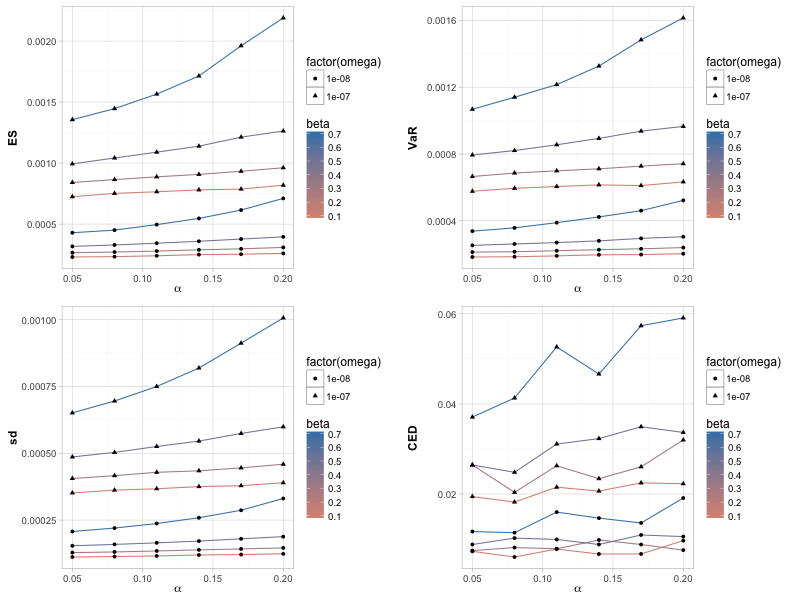
\includegraphics[width = 0.9\textwidth]{../figures/simulation_garch/garch_AR1_risk_measures_neg_alpha.png}
\caption{AR(1): Relationship between $\alpha$ parameter in the GARCH(1,1) and risk measures. The plots are produced under $\kappa_1 = -0.25$. The tend and pattern under $\kappa_1 = 0.25$ is almost the same.}
%(Simulation path length: 1000, $\epsilon_t \sim 0.01T(df = 4)$)
\label{fig:garch_rm_alpha1}
\end{figure}

Figure \ref{fig:garch_rm_coef1} explores the how large $\omega$, $\alpha$ or $\beta$ affect the risk measurements comparing with changing in serial correlation. As proved, we only choose the positive coefficients to see the clear trend. With in $\alpha$ and $\beta$, the $\beta$ is dominant, especially in the first three plots, the 0.5 change in $beta$ is larger than 0.7 change in $\kappa$, fixed $\alpha$. A more exciting pattern shown in the CED plot. It shows that the complex variance, $\alpha$ or $\beta$ less affect CED, comparing the other risk measurements. In general, the curve in last plot is steeper, suggesting that CED is more sensitive to$\kappa$ in AR(1) +GARCH(1,1) model.

\begin{figure}[H]
\centering
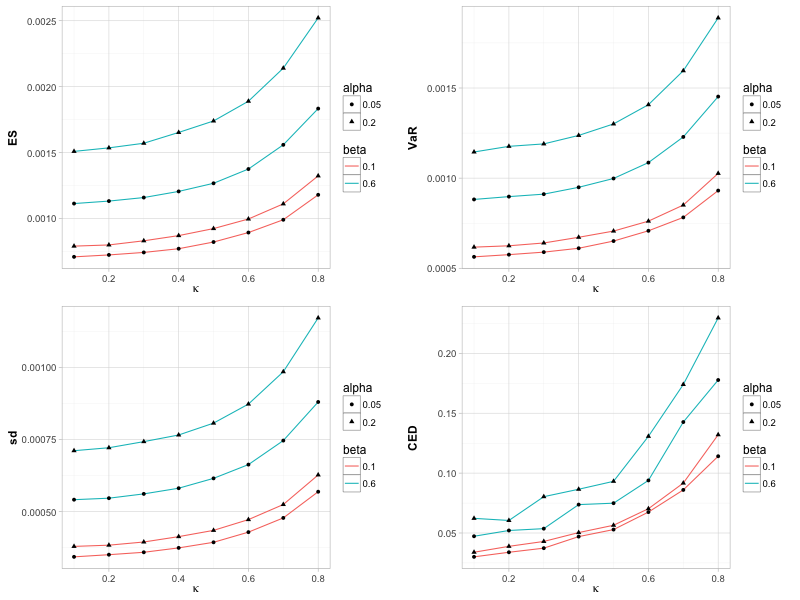
\includegraphics[width = 0.9\textwidth]{../figures/simulation_garch/garch_AR1_risk_measures_ar1}
\caption{AR(1): Relationship between serial correlation in the GARCH(1,1) and risk measures. $\kappa_1 \in \{0.1,0.2, \dots, 0.8 \}$}
%(Simulation path length: 1000, $\epsilon_t \sim 0.01T(df = 4)$)
\label{fig:garch_rm_coef1}
\end{figure}

\begin{figure}[H]
\centering
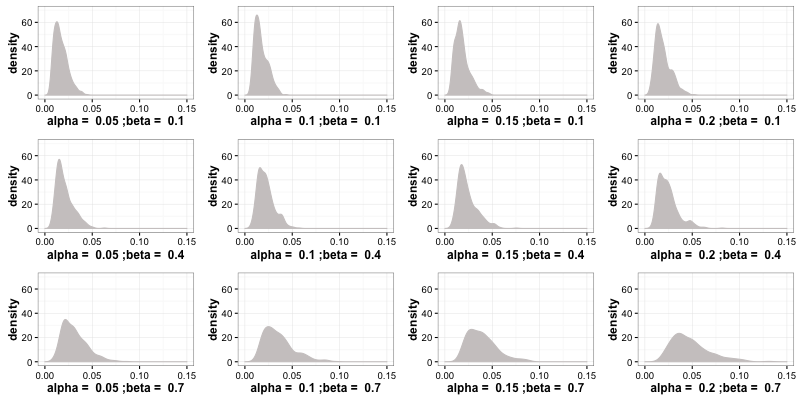
\includegraphics[width = 0.9\textwidth]{../figures/simulation_garch/garch_AR1_alpha_beta}
\caption{AR(1): maximum drawdown distributions under different $\alpha$ and $\beta$. $\kappa = 0.25$, $\omega = 10^{-7}$ is fixed }
%(Simulation path length: 1000, $\epsilon_t \sim 0.01T(df = 4)$)
\label{fig:garch_ar1_ddd}
\end{figure}

Figure \ref{fig:garch_ar1_ddd} show the maximum drawdown distribution's change with the different $\alpha$ and $\beta$. Clearly a higher $\beta$ responsible for a more spread-out distribution, while $\alpha$ is less determinant. Table \ref{table:dist_garch_ar1_return} further confirms this point.

\begin{table}[H]
\centering
\begin{tabular}{|r |r r r r|}
\hline
& Mean & Sd & Skewness & Kurtosis \\
\hline
$\alpha = 0.05 $ & 0.0 & 0.029 & -0.003 & 0.088\\
$\alpha = 0.08 $ & 0.0 & 0.013 & 0.001 & -0.033\\
$\alpha = 0.11 $ & 0.0 & 0.011 & -0.000 & -0.001\\
$\alpha = 0.14 $ & 0.0 & 0.011& -0.004 &  0.006\\
$\alpha = 0.17 $ & 0.0 & 0.013 & -0.014 & -0.004\\
$\alpha = 0.20 $ & 0.0 & 0.029 & 0.005 & 0.054\\
\hline
\end{tabular}
\caption{Statistics of simulated return distribution of AR(1)+ GARCH(1,1)}
\label{table:dist_garch_ar1_return}
\end{table}


%%%%%%%%%%%% MA(1) + GARCH(1,1) %%%%%%%%%%%%%%%%
\subsection{MA(1) + GARCH(1,1)}
There is no much special in need of highlighting comparing with AR(1) + GARCH(1,1) model. Figure \ref{fig:garch_rm_alpha1_ma} and Figure \ref{fig:garch_rm_coef_ma} indicates a similar effect of $omega$, $alpha$ and $\beta$ on risk measurements.  However, at this time, the CED plots is less noisy than that in AR(1) model.

\begin{figure}[H]
\centering
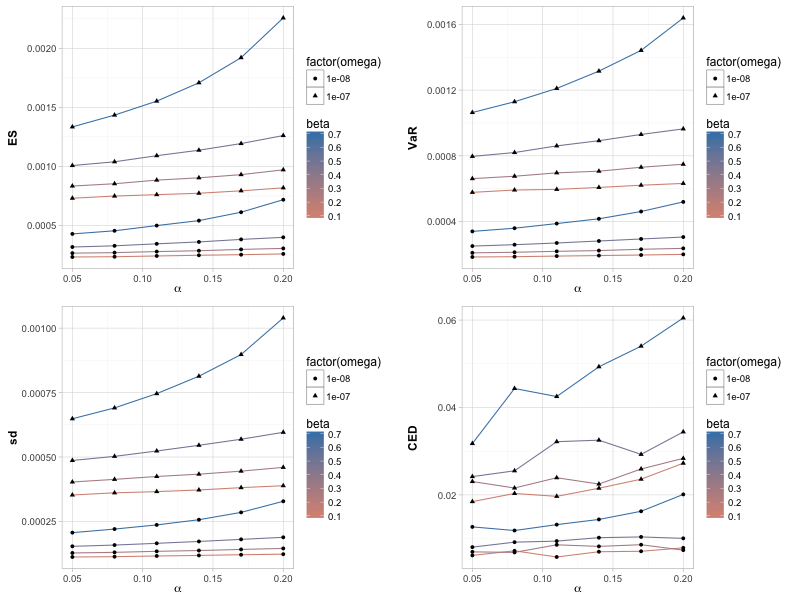
\includegraphics[width = 0.9\textwidth]{../figures/simulation_garch/garch_MA1_risk_measures_neg_alpha.png}
\caption{MA(1): Relationship between $\alpha$ parameter in the GARCH(1,1) and risk measures. The plots are produced under $\theta_1 = -0.25$. The tend and pattern under $\theta_1 = 0.25$ is almost the same.}
%(Simulation path length: 1000, $\epsilon_t \sim 0.01T(df = 4)$)
\label{fig:garch_rm_alpha1_ma}
\end{figure}

\begin{figure}[H]
\centering
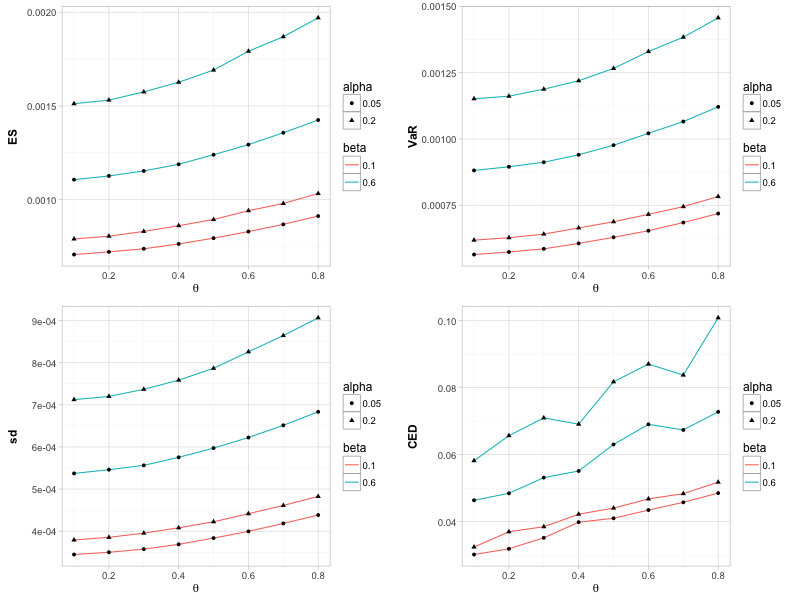
\includegraphics[width = 0.9\textwidth]{../figures/simulation_garch/garch_MA1_risk_measures_ma1}
\caption{MA(1): Relationship between serial correlation in the GARCH(1,1) and risk measures. $\theta_1 \in \{0.1,0.2, \dots, 0.8 \}$}
%(Simulation path length: 1000, $\epsilon_t \sim 0.01T(df = 4)$)
\label{fig:garch_rm_coef_ma}
\end{figure}

\begin{figure}[H]
\centering
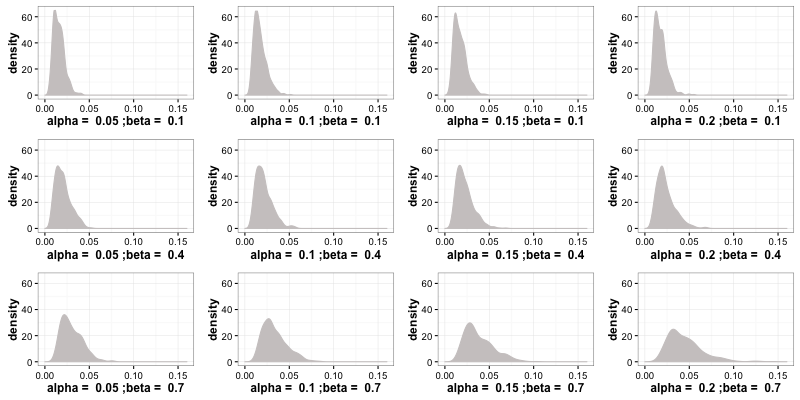
\includegraphics[width = 0.9\textwidth]{../figures/simulation_garch/garch_MA1_alpha_beta}
\caption{MA(1): maximum drawdown distributions under different $\alpha$ and $\beta$. $\theta = 0.25$, $\omega = 10^{-7}$ is fixed }
%(Simulation path length: 1000, $\epsilon_t \sim 0.01T(df = 4)$)
\label{fig:garch_ma1_ddd}
\end{figure}

%%%%%%%%%%%% ARMA(1,1) + GARCH(1,1) %%%%%%%%%%%%%%
\subsection{ARMA(1,1) + GARCH(1,1)}
ARMA(1,1) adds complexity of the model compared with pure AR or MA, while it is also very commonly used in the finance area. We examine the GARCH(1,1) with various GARCH parameters on ARMA(1,1), with $\kappa_1 \in \{0.25, -0.25\}$, $\theta_1 \in \{0.25, -0.25\}$ fixed, thus four combinations in total. Figure \ref{fig:garch_ARMA11_risk_measures_4_alpha} and Figure \ref{fig:garch_ARMA11_risk_measures_3_alpha} are two case showing the extreme difference in CED. The other two cases are put in the appendix later, which are shows a similar pattern as mentioned in the previous section.

\ref{fig:garch_ARMA11_risk_measures_4_alpha} shows when both ARMA parameters are positive, the change $\alpha$ does not add ``trend" in the CED, only more noisy than before.  However, in Figure \ref{fig:garch_ARMA11_risk_measures_3_alpha} where $\kappa_1 = 0.25$, $\theta_1 = -0.25$, the CED increases with the $\alpha$ and more sensitive when $\beta$ is high. Again, the $\omega$ is also the dominant factor compared with $\alpha$ and $\beta$.

\begin{figure}[H]
\centering
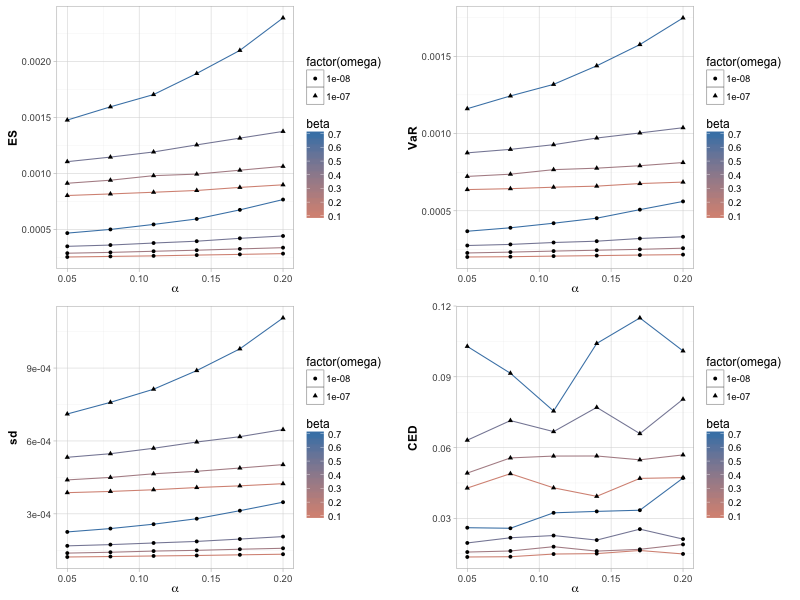
\includegraphics[width = 0.9\textwidth]{../figures/simulation_garch/garch_ARMA11_risk_measures_4_alpha}
\caption{ARMA(1,1): Relationship between $\alpha$ parameter in the GARCH(1,1) and risk measurements. The plots are produced under $\kappa_1 = 0.25$, $\theta_1 = 0.25$. }
%(Simulation path length: 1000, $\epsilon_t \sim 0.01T(df = 4)$)
\label{fig:garch_ARMA11_risk_measures_4_alpha}
\end{figure}

\begin{figure}[H]
\centering
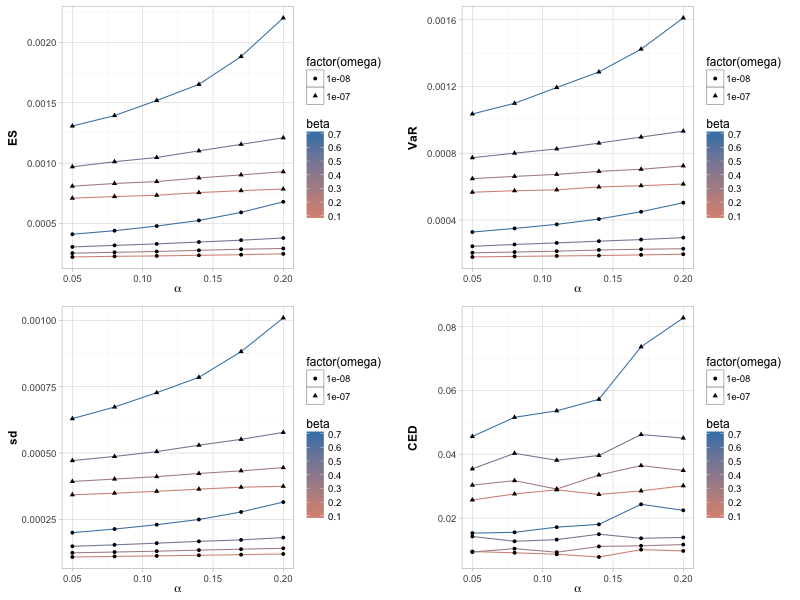
\includegraphics[width = 0.9\textwidth]{../figures/simulation_garch/garch_ARMA11_risk_measures_3_alpha}
\caption{ARMA(1,1): Relationship between $\alpha$ parameter in the GARCH(1,1) and risk measurements. The plots are produced under $\kappa_1 = 0.25$, $\theta_1 = -0.25$. }
%(Simulation path length: 1000, $\epsilon_t \sim 0.01T(df = 4)$)
\label{fig:garch_ARMA11_risk_measures_3_alpha}
\end{figure}

The following the two plots shows the ARMA parameters effects on the risk measurements, and also compare the magnitude with the GARCH parameters. For ES, VaR and volatility, the plots shows that the they are linearly increasing with the $\theta_1$, while non-linearly (probably quadratic, positive first derivative) increasing with the $\kappa_1$. Compared with traditional risk measurements, the plots of CED are more dended. Similarly to the previous conclusions, CED seems to be more sensitive to $\kappa$ and less sensitive to $\theta$. More over, when $\omega$, or the general trend, is small, the CED is very closed for different alpha.

\begin{figure}[H]
\centering
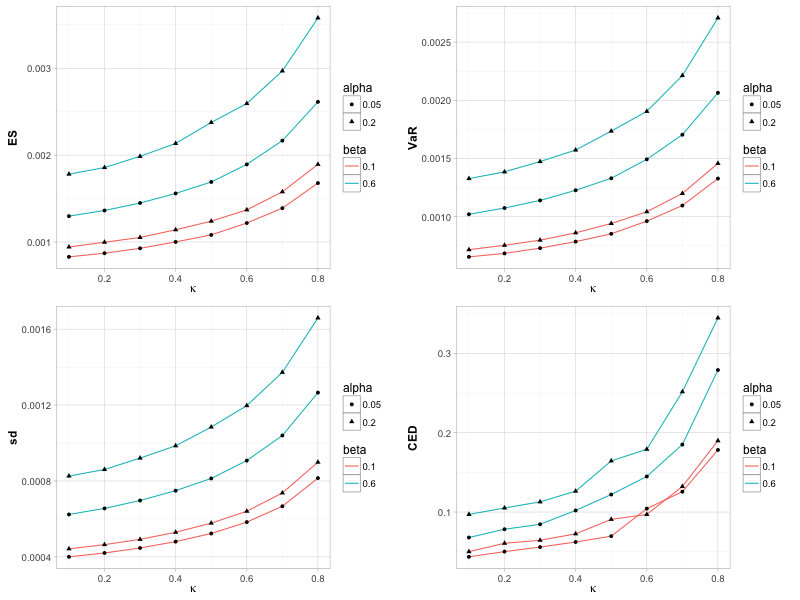
\includegraphics[width = 0.9\textwidth]{../figures/simulation_garch/garch_ARMA11_risk_measures_ar1}
\caption{ARMA(1,1): Relationship between AR coefficients in the GARCH(1,1) and risk measures. $\kappa_1 \in \{0.1,0.2, \dots, 0.8 \}$. The $\omega$  is fixed as $10^{-7}$, and $\theta_1 = 0.5$}
%(Simulation path length: 1000, $\epsilon_t \sim 0.01T(df = 4)$)
\label{fig:garch_rm_coef_ar}
\end{figure}

\begin{figure}[H]
\centering
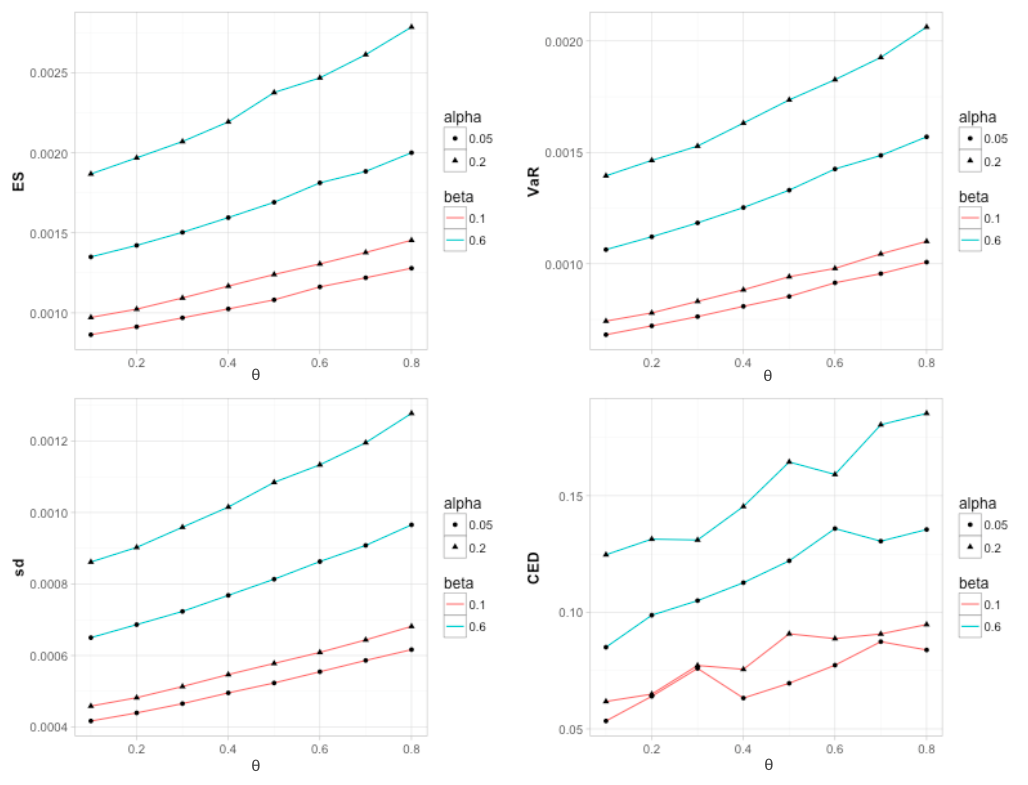
\includegraphics[width = 0.9\textwidth]{../figures/simulation_garch/garch_ARMA11_risk_measures_ma1}
\caption{MA(1): Relationship between MA coefficient in the GARCH(1,1) and risk measures. $\theta_1 \in \{0.1,0.2, \dots, 0.8 \}$. The $\omega$  is fixed as $10^{-7}$, and $\kappa_1 = 0.5$}
%(Simulation path length: 1000, $\epsilon_t \sim 0.01T(df = 4)$)
\label{fig:garch_rm_coef_ma}
\end{figure}


The following is the maximum drawdown distribution for various combination of $\alpha$ and $\beta$. Again, the $\beta$ has a greater effect the distribution comparing with $alpha$. However, it may be partially resulted from we chose $\alpha$ from a smaller range, although it is more close to the real market.

\begin{figure}[H]
\centering
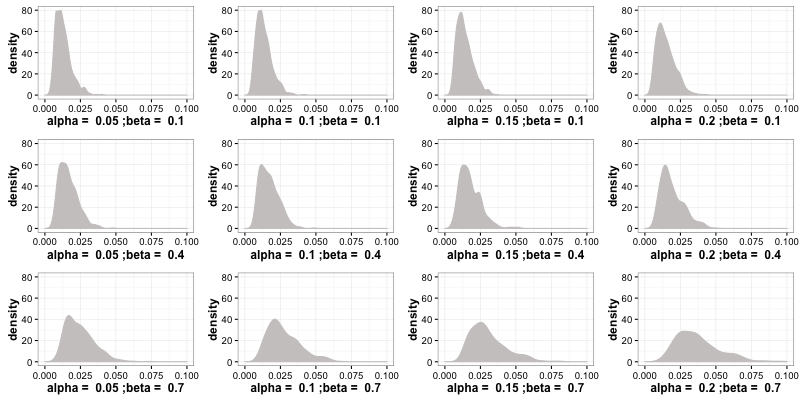
\includegraphics[width = 0.9\textwidth]{../figures/simulation_garch/garch_ARMA11_alpha_beta_3}
\caption{MA(1): maximum drawdown distributions under different $\alpha$ and $\beta$. $\theta = 0.25$, $\omega = 10^{-7}$, $\kappa_1 = 0.25$,$\theta_1 = -0.25$ is fixed }
%(Simulation path length: 1000, $\epsilon_t \sim 0.01T(df = 4)$)
\label{fig:garch_ma1_ddd}
\end{figure}
\subsection{Short Summary about ARMA-GARCH Model}
In this section, we have analyzed the impact of complex variance on the evaluation relationship of serial correlation($\kappa$ or $\rho$) and risk measurements. It is more straightforward to see this effect through the simulation study other than tedious derivations. Through the plots shown above, we have several conclusions as followed.

\begin{enumerate}
\item The larger value of $\omega$, $\alpha$ and $\beta$ are all partially responsible for a higher risk measurements, in general, given the ARMA model.
\item Among three parameters, the effect of $\omega$ dominates. As $\omega$ indicates the general change of variance of the model, which is a counterpart of $\sigma^2$ in the pure ARMA.
\item When the $\beta$ is small, the effect of $\alpha$ on risk measurements are weak. Especially for CED, it is insensitive to the change of $\alpha$. However, when the $\beta$ value is large, the ES, VaR and Volatility increase sharply with $\alpha$. For CED, it has a upward trend, but more indented than other risk measurements.
\item From the plots with $\kappa$ as axis, we found that in the time series with a GARCH variance, $\alpha$ and $\beta$ less affect CED comparing with other risk measurements.
\item Last but not least, we found that $\alpha$ value of the GARCH model does not change the shape of maximun drawdown distribution a lot compare with $\beta$ values. Therefore, in summary, for CED, the ranking magitude of effect from GARCH parameters are: $\alpha < \beta < \omega$
\end{enumerate}

%%%%%%%%%%%%%%%%%%%%%%%%%
\section{Findings}  %%%%%
%%%%%%%%%%%%%%%%%%%%%%%%%

\subsection{Finding 1}

\textbf{CED distinguishes negative from positive autocorrelation}

For time series with positive autocorrelation, return is very likely to have the same sign as the return in the previous day. For example, if return in April 5 is -1\% and there is a positive autocorrelation, the return in April 6 is more likely to be negative rather than positive. As a consequence, returns tend to keep they current profit or loss status for a period of time. If the current status is loss, then unfortunately, the price of the asset may continuously go down, which results in a large CED.

For time series with negative autocorrelation, return is very likely to have the different sign as the return in the previous day. That is, if the the price of one assets goes down in one day, it is more likely that the price would bounce back in the next day, which leads to a small CED. 

However, other risk measures such as VaR, ES and volatility are obtained from the empirical distribution of returns. If we shuffle the return sequence, we would get the same value for VaR, ES, and volatility but not for CED.

Figure \ref{fig:Comparison_pos_neg_autocorrelation} shows the comparison of simulated returns and prices when serial correlation is 0.7 and -0.7. The maximum drawdown of simulated series is 22.76\% and 9.49\% separately. And these two return series have the same VaR, ES and volatility.

\begin{figure}[H]
\centering
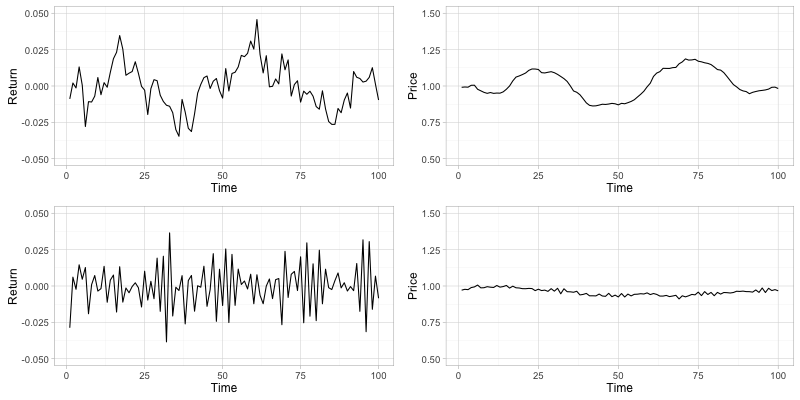
\includegraphics[width = 0.8\textwidth]{../figures/simulation/Comparison_pos_neg_autocorrelation}
\caption{Comparison of returns with positive and negative serial correlation}
(Simulation length: 100; upper panel: AR(1) with $\kappa=0.7$; lower panel: AR(1) with $\kappa=-0.7$, $\epsilon\sim N(0, 0.0001)$)
\label{fig:Comparison_pos_neg_autocorrelation}
\end{figure}

\subsection{Finding 2}

\textbf{Change standard deviation but fix everything in time series simulation would result in linear change of risk measures}

The following simulation result for AR(1) model shows a linear relationship for all risk measures. I simulate the model $X_t = 0.3X_{t-1} + \epsilon_t$ and change the $\epsilon_t$ from 0.001 to 0.015. The simulated path length is 63, which is the number of trading days in three months. 

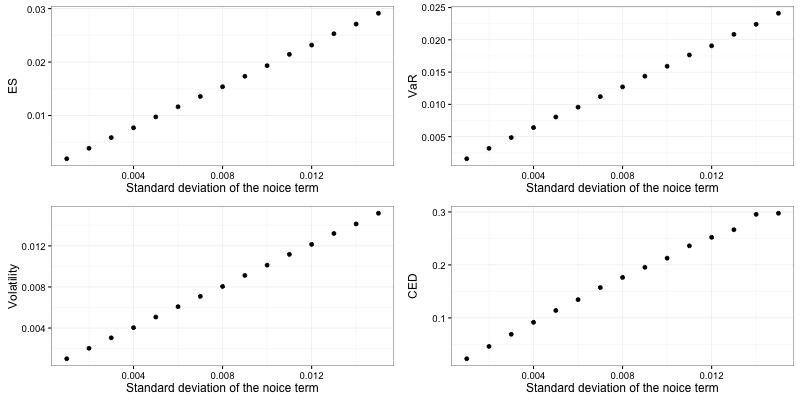
\includegraphics[width = 0.8\textwidth]{../figures/simulation/AR1_risk_measures_change_sd}

This make sense. Fixing everything but changing the standard deviation of the noise term would simply multiply the simulated time series model by a constant. If for $\epsilon_t = 0.001$, we simulated the time series $X_1, X_2, \cdots, X_n$. Then the simulated sequence for $\epsilon_t = 0.01$ would be something like $10X_1, 10X_2, \cdots, 10X_n$. For volatility, ES and VaR, it is easy to see they would be multiplied 10. For CED, I will show below that it would also approximately be multiplied by 10. 

For accumulated returns in a path, the return is approximately the sum of all returns for each day in this time period if the return is small (which is often the case):

\begin{eqnarray}
R & = & \prod_{i=1}^n (1+r_i) - 1\\
& \simeq & \prod_{i=1}^n e^{r_i} - 1 \\
& = & e^{\sum_{i=1}^n r_i} - 1 \\
& \simeq & \sum_{i=1}^n r_i
\end{eqnarray}

Because all the returns in every subpath would be multiplied by approximately 10. Thus the domain of the maximum drawdown distribution and CED would also become 10 times as the counterpart for $\epsilon_t = 0.001$.

%%%%%%%%%%%%%%%%%%%%%%%%%
\section{Thoughts} %%%%%%
%%%%%%%%%%%%%%%%%%%%%%%%%

In the thoughts section above, we focused on the how noise term variance and order 1 serial correlation related with CED. After the simulation of various time series models, we found that CED is correlated with the autocorrelation function. To be more specific, if we simulate two time series model $\{X_t\}$ and $\{Y_t\}$ with the same autocorrelation function $\rho_X(t) = \rho_Y(t)$ for $ t = 0, 1, \cdots, m-1, m+1, \cdots$, but $\rho_X(m) > \rho_Y(m)$, Then the CED of $\{X_t\}$ will be larger than $\{Y_t\}$. However, for real world price data, it is more likely that there will be more complex pattern of the autocorrelation function which results in more complicated variation of CED values. For example, for asset X and asset Y if $\rho_X(1) < \rho_Y(1)$, but $\rho_X(0) > \rho_Y(0)$, it would be harder to decide the relationship between CED of X and CED of Y.

We haven't prove the above idea since simulating two time series with only one term in the autocorrelation function different is hard. But in section 3, we fixed $\rho(0)$ and simulated time series with various $\rho(t), t = 1, 2, \cdots$ and looked at the relationship between $\rho(1)$ and CED. The results are close to what we proposed above. 

\end{document}













